\documentclass[output=paper,colorlinks,citecolor=brown,]{langscibook}
\ChapterDOI{10.5281/zenodo.19708130}
\author{Yvonne Treis\affiliation{CNRS-LLACAN}}

\title{The apprehensive in Kambaata (Cushitic): Form, meaning and origin}


\abstract{Kambaata, a Cushitic language, has a dedicated, fully grammaticalised apprehensive paradigm without known parallels in related or neighbouring languages. This chapter presents an analysis of the morphology, syntax, meaning and origin of the apprehensive. Morphological and syntactic criteria demonstrate its main clause status. Data from a variety of sources show that the apprehensive is employed in direct dialogue. It encodes that a situation is unrealised at reference time, considered possible in the future and judged by the speaker to be undesirable, if not dangerous for any discourse participant. The primary function of the Kambaata apprehensive, in any person, is to express warnings to the addressee, who is alerted to avert the danger. Apprehensive forms of the first person may also serve as a threat. In the second person, the apprehensive has come to express prohibition. Based on detailed language-internal evidence, this chapter demonstrates that the apprehensive paradigm is likely to have resulted from the fusion of a periphrastic verb form in the recent history of the language. The source construction consisted of an affirmative same subject purposive converb plus the existential copula and may have first served to express intentional\slash imminent future.}
  

\IfFileExists{../localcommands.tex}{%hack to check whether this is being compiled as part of a collection or standalone
   \addbibresource{../localbibliography.bib}
   \usepackage{tabularx,multicol}
\usepackage{url}
\urlstyle{same}

\usepackage{langsci-optional}
\usepackage{langsci-lgr}
\usepackage{langsci-gb4e}

\babelprovide[import]{hebrew}

\usepackage{paralist} %%may not be needed, currently used in questionnaire


%Siena added packages for introduction; not sure they are needed
\usepackage[normalem]{ulem}
\useunder{\uline}{\ul}{}

%from Treis:
\usepackage{listings}
\lstset{basicstyle=\ttfamily,tabsize=2,breaklines=true}

%%from Francez
% % % \usepackage{cjhebrew}
%\usepackage{tipa}  Also included by D&A, need to check with LSP whether to change it to language science tipa
\usepackage{leipzig}
%%from Dabkowski&AnderBois:

\usepackage[shortlabels]{enumitem} 
\usepackage{centernot}
\usepackage{arydshln}
\usepackage{newunicodechar}
\usepackage{csquotes}
%\let\sups\relax \usepackage{tipa} commented out on 7/3/25 Martina
% \usepackage[all]{nowidow}
\usepackage{listings} \lstset{basicstyle=\ttfamily}
\usepackage{multirow}
\usepackage{rotating}
\usepackage{pdflscape}
\usepackage{xspace}
%\usepackage{tabularx}
%\usepackage{multicol}
\usepackage{supertabular}
\usepackage{hhline}
\usepackage{bbding} %this package is for the checkmarks in Table 6 in Browne et al.

%\usepackage{qtree}
%\usepackage{tree-dvips}

\usepackage{array}
\usetikzlibrary{calc,tikzmark,matrix}
\usepgflibrary{shadings}
\usepackage{pifont}
%from Fedotov:

\usepackage{langsci-textipa}
%\usepackage{multirow}


%\usepackage{xeCJK}

%%%%%%%%%%%%%%%%%%%%%%%%%%%%%%%%%%%%%%%%%%%%%%%%%%%%
%%% EXAMPLES %%%%%%%%%%%%%%%%%%%%%%%%%%%%%%%%%%%%%%%
%%%%%%%%%%%%%%%%%%%%%%%%%%%%%%%%%%%%%%%%%%%%%%%%%%%% 

% if you want the source line of examples to be in
% italics, uncomment the following line
\renewcommand{\exfont}{\itshape}
% to add additional information to the right of
% examples, uncomment the following line

%\usepackage{langsci/styles/jambox}


%%% FOOTNOTE EXAMPLE NUMBERING
% \makeatletter
% \patchcmd{\@footnotetext}{\setcounter{fnx}{0}}{\renewcommand{\thexnumi}{\roman{xnumi}}}{}{}
% \apptocmd{\@footnotetext}{
%     \@noftnotetrue
%     \renewcommand{\thexnumi}{\arabic{xnumi}}%
% }{}{}
%
% \makeatother
\usepackage[linguistics,edges]{forest}
\usepackage{hyphenat}
\usepackage{langsci-branding}

   \makeatletter
\let\thetitle\@title
\let\theauthor\@author
\makeatother

\newcommand{\togglepaper}[1][0]{
   \bibliography{../localbibliography}
   \papernote{\scriptsize\normalfont
     \theauthor.
     \titleTemp.
    To appear in:
    Martina Faller,  Marine Vuillermet \&  Eva Schultze-Berndt (eds.). Apprehensional Constructions in a cross-linguistic perspective. Berlin: Language Science Press. [preliminary page numbering]
   }
   \pagenumbering{roman}
   \setcounter{chapter}{#1}
   \addtocounter{chapter}{-1}
}

\newbool{bookcompile}
\booltrue{bookcompile}
\newcommand{\bookorchapter}[2]{\ifbool{bookcompile}{#1}{#2}}


\newfontfamily\FedotovBoldEmptySetFont{LibertinusSerif-Italic.otf}[AutoFakeBold=2.5]
\newcommand{\FedotovBoldEmpty}{{\FedotovBoldEmptySetFont\bfseries ∅}}

%From Dabkowski&AnderBois


\let\sc\scshape
\let\rm\rmfamily
%\let\it\itshape
\let\tt\ttfamily
\let\nr\normalfont

\newcommand{\wsc}[1]{\textls[80]{\scshape#1}}

\let\textai\textit
% \let\textlc\spacedlowsmallcaps
% \let\textac\spacedallcaps
\let\textlc\textsc
\let\textac\textsc


%%%%%%%%%%%%%%%%%%%%%%%%%%%%%%%%%%%%%%%%%%%%%%%%%%%%
%%% FLAG %%%%%%%%%%%%%%%%%%%%%%%%%%%%%%%%%%%%%%%%%%%
%%%%%%%%%%%%%%%%%%%%%%%%%%%%%%%%%%%%%%%%%%%%%%%%%%%%

% \newcommand{\scott}  [1]{\textcolor{violet}{#1}}
% \newcommand{\maks}   [1]{\textcolor{blue}{#1}}
% % \newcommand{\data}   [1]{\textcolor{teal}{#1}}
% \newcommand{\new}   [1]{#1}
% \newcommand{\newnew}   [1]{\textcolor{teal}{#1}}
% \newcommand{\rev}   [1]{\textcolor{magenta}{#1}}



%%%%%%%%%%%%%%%%%%%%%%%%%%%%%%%%%%%%%%%%%%%%%%%%%%%%
%%% TABLES %%%%%%%%%%%%%%%%%%%%%%%%%%%%%%%%%%%%%%%%%
%%%%%%%%%%%%%%%%%%%%%%%%%%%%%%%%%%%%%%%%%%%%%%%%%%%%

%\newcolumntype{Y}{>{\arraybackslash}p{25.3543464286pt}} % length of L

% \newcolumntype{K}{>{\arraybackslash}p{24.25pt}}
% \newcolumntype{V}{>{\arraybackslash}p{(\textwidth/9-24pt)/2}}
%
\let\ch\relax \newcommand{\ch}[2]{\multicolumn{#1}{c}{\sc#2}}
\let\sx\relax \newcommand{\sx}[2]{\multicolumn{#1}{l}{\emph{-#2}}} % suffix
\let\su\relax \newcommand{\su}{\sx{1}} % suffix unicolumnal
\let\sd\relax \newcommand{\sd}{\sx{2}} % suffix dicolumnal
\let\cx\relax \newcommand{\cx}[2]{\multicolumn{#1}{l}{\emph{=#2}}} % clitic
\let\cu\relax \newcommand{\cu}{\cx{1}} % clitic unicolumnal
\let\cd\relax \newcommand{\cd}{\cx{2}} % suffix dicolumnal
\let\gx\relax \newcommand{\gx}[2]{\multicolumn{#1}{l}{\sc #2}} % gloss
\let\gd\relax \newcommand{\gd}{\gx{2}} % gloss dicolumnal
\let\gr\relax \newcommand{\gr}[1]{\multicolumn{2}{c}{\multirow{2}{*}{\textcolor{gray}{\sc#1}}}}
\let\db\relax \newcommand{\db}[1]{\multicolumn{2}{c}{\multirow{2}{*}{\sc#1}}}



%%%%%%%%%%%%%%%%%%%%%%%%%%%%%%%%%%%%%%%%%%%%%%%%%%%%
%%% EXAMPLES %%%%%%%%%%%%%%%%%%%%%%%%%%%%%%%%%%%%%%%
%%%%%%%%%%%%%%%%%%%%%%%%%%%%%%%%%%%%%%%%%%%%%%%%%%%%

%%% AFFIX BOUNDARY %%%%%%
% \DeclareRobustCommand{\longmn}{\textminus}
% \DeclareRobustCommand{\mn}{-}

%%% CLITIC BOUNDARY %%%%%%
% \DeclareRobustCommand{\longeq}{=}
% \makeatletter\DeclareRobustCommand{\eq}{%
%     \settowidth{\@tempdima}{-}% width of a hyphen
%     \resizebox{\@tempdima}{\height}{=}%
% }\makeatother

%%% FUZZY CLITIC %%%%%%
% \DeclareRobustCommand{\longfc}{%
%     $\overset{\text{\smash{}}}{\text{$\approx$}}$%
% }
% \makeatletter\DeclareRobustCommand{\fc}{%
%     \settowidth{\@tempdima}{-}% width of a hyphen
%     \resizebox{\@tempdima}{\height}{%
%         $\overset{\text{\smash{}}}{\text{$\approx$}}$%
%     }%
% }\makeatother

%%% REDUPLICATION %%%%%%%
% \DeclareRobustCommand{\longtl}{$\sim$}
% \makeatletter\DeclareRobustCommand{\tl}{%
%     \settowidth{\@tempdima}{-}% width of a hyphen
%     \resizebox{\@tempdima}{\height}{$\sim$}%
% }\makeatother

% \newcommand{\mn}          {\textminus}
\newcommand{\src}    [1]  {\jambox[0pt]{\rm(#1)}}
% \newcommand{\ai}     [2]  {\emph{#1} `\textsc{#2}#3'\xspace}
\newcommand{\ai}     [2]  {\emph{#1} `\textsc{#2}'\xspace}
\newcommand{\sane}   [1][]{\ai{=sa'ne}{appr}{#1}}
\newcommand{\srcn}   [1][]{\ai{kûintsû}{srcn}{#1}}
% \newcommand{\mbekane}[1][]{\ai{\eq mbe kañe}{neg.adv aux.inf}{#1}}

% \let\sc\relax \newcommand{\sc}{\normalfont\scshape}
% \let\rm\relax \newcommand{\rm}{\normalfont\rmfamily}
% \let\it\relax \newcommand{\it}{\normalfont\itfamily}

\newcommand{\lb}{{\rm[}}
\newcommand{\rb}{{\rm]}}

\newcommand{\bad}{\makebox[0pt][r]{*\,}}
\newcommand{\infel}{\makebox[0pt][r]{\#\,}}


% \newcommand{\lsqz}[1]{#1}
% \newcommand{\lsqz}[1]{\makebox[0pt][l]{#1}}

% \newcommand{\lsqu}[1]{\makebox[0pt][l]{#1}}
% \newcommand{\rsqu}[1]{\makebox[0pt][r]{#1}}
% \newcommand{\astr}{\makebox[0pt][r]{{\nr*}}}
% \newcommand{\hash}{\makebox[0pt][r]{{\nr\#}}}
% \newcommand{\qstn}{\makebox[0pt][r]{{\nr?}}}
% \newcommand{\bad}{\makebox[0pt][r]{*}}
% \newcommand{\unhappy}{\makebox[0pt][r]{\#}}


%%%%%%%%%%%%%%%%%%%%%%%%%%%%%%%%%%%%%%%%%%%%%%%%%%%%
%%% UNICODE CHARACTERS  %%%%%%%%%%%%%%%%%%%%%%%%%%%%
%%%%%%%%%%%%%%%%%%%%%%%%%%%%%%%%%%%%%%%%%%%%%%%%%%%%

\newunicodechar{⟨}{⟨}
\newunicodechar{⟩}{⟩}

\newcommand{\infix}{⟨}
\newcommand{\outfix}{⟩}



%%%%%%%%%%%%%%%%%%%%%%%%%%%%%%%%%%%%%%%%%%%%%%%%%%%%
%%% IPA %%%%%%%%%%%%%%%%%%%%%%%%%%%%%%%%%%%%%%%%%%%%
%%%%%%%%%%%%%%%%%%%%%%%%%%%%%%%%%%%%%%%%%%%%%%%%%%%%

% \newcommand{\ipa}{\textipa}

\newcommand{\sub}{\textsubscript}
% \let\super\relax \newcommand{\super}{\textsuperscript}

\newcommand{\ts}{\texttslig}
% \let\dz\relax \newcommand{\dz}{\textdzlig}
\newcommand{\tS}{\textteshlig}
\newcommand{\dZ}{\textdyoghlig}
\newcommand{\cj}{\textctc}
\newcommand{\sj}{\textctc}
\newcommand{\zj}{\textctz}
\newcommand{\tcj}{\texttctclig}
\newcommand{\tsj}{\texttctclig}
\newcommand{\dzj}{\textdctzlig}
\newcommand{\gj}{\textbardotlessj}
% \let\nj\relax \newcommand{\nj}{\textltailn}
% \newcommand{\W}{\textturnmrleg}
\newcommand{\wl}{\textturnmrleg}
% \newcommand{\1}{\ipabar{\~\i}{.5ex}{1.1}{}{}}
\newcommand{\dotlessibar}{\ipabar{\i}{.5ex}{1.1}{}{}}
\newcommand{\darkl}{\textltilde}
% \newcommand{\n}{\textsubarch}
% \newcommand{\x}{\textovercross}
\newcommand{\lowered}{\textlowering}
\newcommand{\raised}{\textraising}
\newcommand{\retracted}{\textsubbar}
\newcommand{\unreleased}{\textcorner}
% \newcommand{\syllabic}{\s}
\newcommand{\implosivet}{\texthtt}
\newcommand{\implosived}{\texthtd}
\newcommand{\implosivep}{\texthtp}
\newcommand{\implosiveb}{\texthtb}
\newcommand{\implosivek}{\texthtk}
\newcommand{\implosiveg}{\texthtg}



%%%%%%%%%%%%%%%%%%%%%%%%%%%%%%%%%%%%%%%%%%%%%%%%%%%%
%%% OTHER %%%%%%%%%%%%%%%%%%%%%%%%%%%%%%
%%%%%%%%%%%%%%%%%%%%%%%%%%%%%%%%%%%%%%%%%%%%%%%%%%%%

\newcommand{\ie}{i.\,e.\xspace}
\newcommand{\Ie}{I.\,e.\xspace}
\newcommand{\eg}{e.\,g.\xspace}
\newcommand{\Eg}{E.\,g.\xspace} 




\newcommand{\francoissource}[1]{\hfill\textnormal{{\footnotesize #1} }}
\newcommand{\E}{Ɛ\kern-1.5pt\raisebox{1pt}{̏}\kern1.5pt}
\newcommand{\ù}{{ṵ}\kern-2pt{̀}\kern2pt}
\newcommand{\ȕ}{{ṵ}\kern-2pt{̏}\kern2pt}

\newcommand{\OO}{ɔ\kern-1pt\raisebox{-1pt}{̰}\kern1pt}
\newcommand{\Ǒ}{{{ɔ̌\kern-1pt\raisebox{-.5pt}{̰}\kern1pt}}}


\newcommand{\à}{{a̰}\kern-2pt{̀}\kern2pt}
\newcommand{\ilit}[1]{#1\il{#1}}

   %% hyphenation points for line breaks
%% Normally, automatic hyphenation in LaTeX is very good
%% If a word is mis-hyphenated, add it to this file
%%
%% add information to TeX file before \begin{document} with:
%% %% hyphenation points for line breaks
%% Normally, automatic hyphenation in LaTeX is very good
%% If a word is mis-hyphenated, add it to this file
%%
%% add information to TeX file before \begin{document} with:
%% %% hyphenation points for line breaks
%% Normally, automatic hyphenation in LaTeX is very good
%% If a word is mis-hyphenated, add it to this file
%%
%% add information to TeX file before \begin{document} with:
%% \include{localhyphenation}

\hyphenation{
par-a-digm
com-ple-men-ta-tion
anaph-o-ra
Dor-drecht
Cu-shi-tic
be-ne-dic-tive
pa-ra-digms
Ethi-o-pi-an
hoch-land-ost-ku-schi-ti-schen 
Duu-raa-me
Pa-ken-dorf
Lich-ten-berk
affri-ca-te
affri-ca-tes
com-ple-ments
Eng-lish
}




\hyphenation{
par-a-digm
com-ple-men-ta-tion
anaph-o-ra
Dor-drecht
Cu-shi-tic
be-ne-dic-tive
pa-ra-digms
Ethi-o-pi-an
hoch-land-ost-ku-schi-ti-schen 
Duu-raa-me
Pa-ken-dorf
Lich-ten-berk
affri-ca-te
affri-ca-tes
com-ple-ments
Eng-lish
}




\hyphenation{
par-a-digm
com-ple-men-ta-tion
anaph-o-ra
Dor-drecht
Cu-shi-tic
be-ne-dic-tive
pa-ra-digms
Ethi-o-pi-an
hoch-land-ost-ku-schi-ti-schen 
Duu-raa-me
Pa-ken-dorf
Lich-ten-berk
affri-ca-te
affri-ca-tes
com-ple-ments
Eng-lish
}


 
   \boolfalse{bookcompile}
    \togglepaper[23]
}{}


\begin{document}
\maketitle
%\shorttitlerunninghead{}%%use this for an abridged title in the page headers

%%Note to editors
%%Please copy information from localhyphenation.tex
%%Please do not change the order of names of Ethiopian authors in localbibliography.bib (Ethiopians have no family names and are quoted by their first name).
%Still to be added: Cross-references to other chapters in the book
%Formatting of tables still needs to be adapted to page width.

\section{Introduction}\label{sec:treis:1}

This chapter presents a detailed analysis of the fully grammaticalised apprehensive main verb paradigm in \ili{Kambaata},\footnote{Iso-code 639-3: \href{https://iso639-3.sil.org/code/ktb} {ktb}, Glottolog code: \href{https://glottolog.org/resource/languoid/id/kamb1316} {kamb1316}.} a \ili{Cushitic} language of Ethiopia. The apprehensive, as illustrated by \textit{agókkookke} `it might drink you, it might make you drown' in (\ref{ex:treis:1}) and \textit{eebbókkoont} `you might bring' in (\ref{ex:treis:2}), expresses apprehension on the part of the speaker that a potential, undesirable situation may arise and serves as a warning to the addressee. The addressee is alerted so that they take care or counteract any adverse effects. The apprehensive is often translated as negative (`beware that \textsc{subject} does not \textsc{verb}') but does not contain any overt negative morphology.

\ea\label{ex:treis:1} 
\gll Wó'-u ag-\textbf{ókkoo}-kke! \\
water-\textsc{m.nom} drink-\textsc{3m.appr-2sg.obj}\\
\glt (Husband alerts his wife when approaching a dangerous river) `(Watch out!) The water might ``drink'' you. / Beware that the water does not ``drink'' you (i.e.\ that you don't drown).' [Dialogue in a narrative, Field notes 2004]
\z

\ea\label{ex:treis:2}
\gll Aador-á			úl-t				tíg-unta.\\
rock-\textsc{m.acc} touch-\textsc{3m.pfv.cvb} tumble.down-\textsc{3m.purp.ds}\\ \newline
\gll áabb-a,		eeb-\textbf{bókkoont} reh-úta! \\
son-\textsc{m.voc}	bring-\textsc{2sg.appr} 	death-\textsc{f.acc}\\
\glt (In a playful competition, a girl warns a flirty boy of undesirable consequences of his advances) `(Watch out!) When you touch the rocks and cause a landslide, (my) son, you might bring death!' / `Don't touch the rocks to cause a landslide, (my) son, and (thus) bring death!' (Double entendre, Alemu Banta, personal communication, 2019)\footnotemark]
\z
\footnotetext{Genre: \textit{Qaanqúta} `double entendre'. Note the alliteration and the rhyme.}

\ili{Kambaata} is one of only two known African languages with a dedicated main verb form for warnings and threats (see \citealt{chapters/fedotov} on the apprehensive construction in the \ili{Mande} language \ili{Gban}).\footnote{As pointed out to me by Ronny Meyer (personal communication, 2020), \ili{Muher}, an \ili{Ethiosemitic} language of the \ili{Gunnän Gurage} branch, may also have a yet undescribed dedicated apprehensive paradigm. \ili{Muher} is unrelated to \ili{Kambaata} but spoken in the proximity of \ili{Highland East Cushitic} languages in southwestern Ethiopia.} This chapter envisages a detailed synchronic and diachronic description of the \ili{Kambaata} apprehensive based on field notes and data from local publications. The first section of this chapter is a brief introduction into the language; it provides information on its classification, sociolinguistic aspects and official orthography (\sectref{sec:treis:1.1}) and on typological features (\sectref{sec:treis:1.2}). In \sectref{sec:treis:1.3}, the type of linguistic data used for this study and the number of occurrences of apprehensive examples in the corpus are tabulated. \sectref{sec:treis:2} is dedicated to formal aspects of the apprehensive paradigm: \sectref{sec:treis:2.1} discusses where the apprehensive fits into the typology of \ili{Kambaata} verb forms, while \sectref{sec:treis:2.2} analyses the individual apprehensive forms and explains their morphological makeup. Semantic aspects of the apprehensive are the focus of \sectref{sec:treis:3}, which divides into sections on third, first and second person forms (\sectref{sec:treis:3.1}-\sectref{sec:treis:3.3}). The syntax of apprehensive sentences and the expression of pre-emptive measures are elaborated on in \sectref{sec:treis:4}. Finally, \sectref{sec:treis:5} traces the historical development from a periphrastic imminent future verb to an apprehensive on the basis of detailed language-internal evidence. The paper is concluded in \sectref{sec:treis:6}.

Terminological note: In earlier publications and conference papers on \ili{Kambaata}, I have glossed and labelled the verb forms for warning and threats in various ways. As I was unsure about the functional range and typological parallels of the \nobreakdash-\textit{ókkoo}-paradigm, I was torn between the labels ``intimidative'', ``admonitive'', ``preventive'' and ``advertive''. The comparison with functionally equivalent verb forms in other languages shows that ``apprehensive'' is the most appropriate name for the \nobreakdash-\textit{ókkoo}-paradigm.

\subsection{Classification, sociolinguistics and orthography}\label{sec:treis:1.1}

\ili{Kambaata} (endonym: \textit{Kambaatissáta}) is a \ili{Cushitic} language of the \ili{Afroasiatic} phylum. Together with six other languages it constitutes the \ili{Highland East Cushitic} language group; \ili{Alaaba} and \ili{K'abeena} are its closest relatives. \ili{Kambaata} is spoken in southwestern Ethiopia in the Kambaata-Xambaaro Zone of the Southern Nation, Nationalities, and Peoples' Region, about 300km's distance from the Ethiopian capital Addis Ababa. According to the last census data \citep[91]{CSA2007}, the language has (at least) 615,000 speakers. \ili{Amharic}, the Ethiopian lingua franca and federal working language, is the most important second language of \ili{Kambaata} speakers. 

The official \ili{Kambaata} orthography is based on the Roman script (\citealt[73--80]{Treis2008}; \citealt{Alemu2016}) and is largely phonemic: It represents the 5 vowel and 27 consonant phonemes as well as phonemic length. In this contribution, the official orthography is adopted with only minor adaptations: phonemic stress is consistently marked throughout the paper by an acute accent, and the phonemic glottal stop is consistently written wherever it occurs in word-medial and word-final position. The following graphemes of the official orthography are not in accordance with the IPA conventions: <ph> /p'/, <x> /t'/, <q> /k'/, <j> /dʒ/, <c> /tʃ'/, <ch> /tʃ/, <sh> /ʃ/, <y> /j/ and <'> /Ɂ/. Geminate consonants and long vowels are marked by doubling,  e.g.\ <shsh> /ʃ:/ and <ee> /e:/. Consonant clusters consisting of a glottal stop and a sonorant are written as trigraphs,  e.g.\ <'rr> /Ɂr/, to distinguish them from laryngealised sonorants,  e.g.\ <'r> /r'/.

\subsection{Typological profile}\label{sec:treis:1.2}

\ili{Kambaata} is an agglutinating-fusional language and strictly suffixing. Its constituent order is head-final; hence all modifiers precede the noun in the noun phrase, and all dependent clauses precede independent main clauses. The last constituent in a sentence is usually a fully finite verb or a copula.\footnote{In poetry -- see  e.g.\ (\ref{ex:treis:2}) -- the word order is more flexible.} The following open word classes can be defined on morphosyntactic grounds: nouns, adjectives, verbs, ideophones and interjections. The word class of adverbs is marginal, there are a small number of independent discourse markers, no adpositions and only two true conjunctions. \ili{Kambaata} is head- and dependent-marking with an elaborate case system and subject indexing on verbs. The case system is nominative-accusative: The nominative marks the grammatical subject, whereas the accusative marks direct objects and certain adverbial constituents and serves as the citation form. Nouns and certain pronouns distinguish nine case forms,\footnote{None of these case forms is used with apprehensional meanings.} all of which are marked by a segmental suffix and a specific stress pattern; the case system of adjectives is reduced to three forms (accusative, nominative, oblique). Nouns, pronouns and adjectives are not only obligatorily marked for case but also for gender (masculine vs.\ feminine). The assignment of gender is mostly arbitrary and only sex-based in the case of nouns referring to human beings and higher animals. Adjectives are a macro-word class of case-\slash gender\hyp agreeing lexemes that also encompasses cardinal numerals and adnominal demonstratives. Pronouns form a heterogeneous closed word class that subdivides into personal, interrogative and demonstrative pronouns. Ideophones and interjections are morphologically invariant. The former are syntactically integrated and inflected with the help of light verbs (\textit{y}- `say', \textit{ih}- `become', \textit{ass}- \~{} \textit{a'}- `do'), the latter constitute utterances of their own. Major features of the verbal system are highlighted in \sectref{sec:treis:2} to compare the morphology of the apprehensive with that of other verb forms.

\subsection{Data}\label{sec:treis:1.3}
\largerpage
My corpus contains altogether 136 apprehensive examples, which come from a variety of sources that were collected since 2002: recorded conversations and stories, overheard examples, solicited mock dialogues, elicited data and local publications (see \tabref{tab:treis:1}).\footnote{The written sources consulted are: \citet{Saint-Exupéry2018}; schoolbooks: \citet[grade 1--8]{KEB1989}, (\citeyear[grade 9--10]{KEB2007}), (\citeyear[grade 1--4]{KEB2008a}), (\citeyear[grade 11]{KEB2008b}) and (\citeyear[grade 12]{KEB2010}); biblical and religious texts: \citet{KHTPH2005} and (\citeyear{KHTPHNodate}), and \citet{BrookYonathan2013}; dictionary: \citet{Alemu2016}; proverb collection: \citet{AlamuAlamaayyo2017}.}   
\clearpage

\begin{table}
\caption{Sources of apprehensive examples}
\label{tab:treis:1}
 \begin{tabular}{lrrrr}
  \lsptoprule
            & 1\textsuperscript{st} person & 2\textsuperscript{nd} person & 3\textsuperscript{rd} person & All\\
  \midrule
Recorded: Conversations & - & 2 & 1 & 3\\
Recorded: Stories & - & - & 1 & 1\\
Field notes: Overheard & - & 4 & - & 4\\
Field notes: Mock dialogues & 3 & 5 & 13 & 21\\
Field notes: Elicitation & 12 & 17 & 19 & 48\\ 
Written: Little Prince & - & 7 & 1 & 8\\
Written: Schoolbooks & 2 & 27 & 11 & 40\\
Written: Gospel of John & - & 1 & - & 1\\
Written: Deuteronomy (ms.) & - & 1 & 5 & 6\\
Written: Religious text & - & 1 & - & 1\\
Written: Dictionary & - & 1 & 1 & 2\\
Written: Proverb collection & - & - & 1 & 1\\
  \midrule
  Total & 16 & 66 & 53 & \textbf{136}\\
  \lspbottomrule
 \end{tabular}
\end{table}


Mock dialogues are dialogues of a small number of turns (often 2--4) that are invented by a native speaker under minimal meta-language influence. The speaker is either given a certain communicative setting in English, as in (\ref{ex:treis:3}), or a \ili{Kambaata} word form as a point of departure, as in (\ref{ex:treis:4}).

\ea\label{ex:treis:3} \textnormal{Example instruction}\\
\textnormal{Imagine a natural dialogue between a mother and a daughter about a dangerous situation for their chicken. (For the apprehensive form thus obtained see (\ref{ex:treis:27}).)}
\z

\ea\label{ex:treis:4} \textnormal{Example instruction}\\
\textnormal{Imagine a natural dialogue between two people in which the word form \textit{osa'llókkoombe} (= \textsc{2sg.appr} of \textit{osa'll}- `laugh') is naturally used by one of the speakers. (For the example sentence thus obtained see (\ref{ex:treis:11}).)}
\z

Elicited data was prompted by apprehensive examples extracted from oral and written texts, or examples sentences were generated by native speakers after I had proposed potential verb forms to them. Elicited examples are also found as by-products in questionnaires on the tense-aspect system or on subordination. The elicited examples were discussed with native speakers to solicit descriptions of possible natural contexts in which they could occur. Most of the data on which this contribution is based was again verified during a field trip in February 2019.

\section{Morphology}\label{sec:treis:2}
\subsection{The apprehensive in the typology of Kambaata verbs forms}\label{sec:treis:2.1}

\ili{Kambaata} makes a primary morphological distinction between verbs that are used in main vs.\ subordinate clauses (\figref{fig:treis:1}). Fully finite main verbs sub-divide into indicative and directive verb forms. Indicative main verb forms are marked for four different aspects.\footnote{Tense is not an inflectional category of the \ili{Kambaata} verb system. The post-predicate particle \textit{íkke} is used to mark past tense (if not clear from the linguistic context) or counterfactuality.} The directive is unmarked for aspect and splits up into imperative, jussive and benedictive moods. As the apprehensive is exclusively used as a final verb in main clauses and can as such govern all types of subordinate clauses (\sectref{sec:treis:4}), it definitely belongs to the class of main verbs.

\begin{figure}
    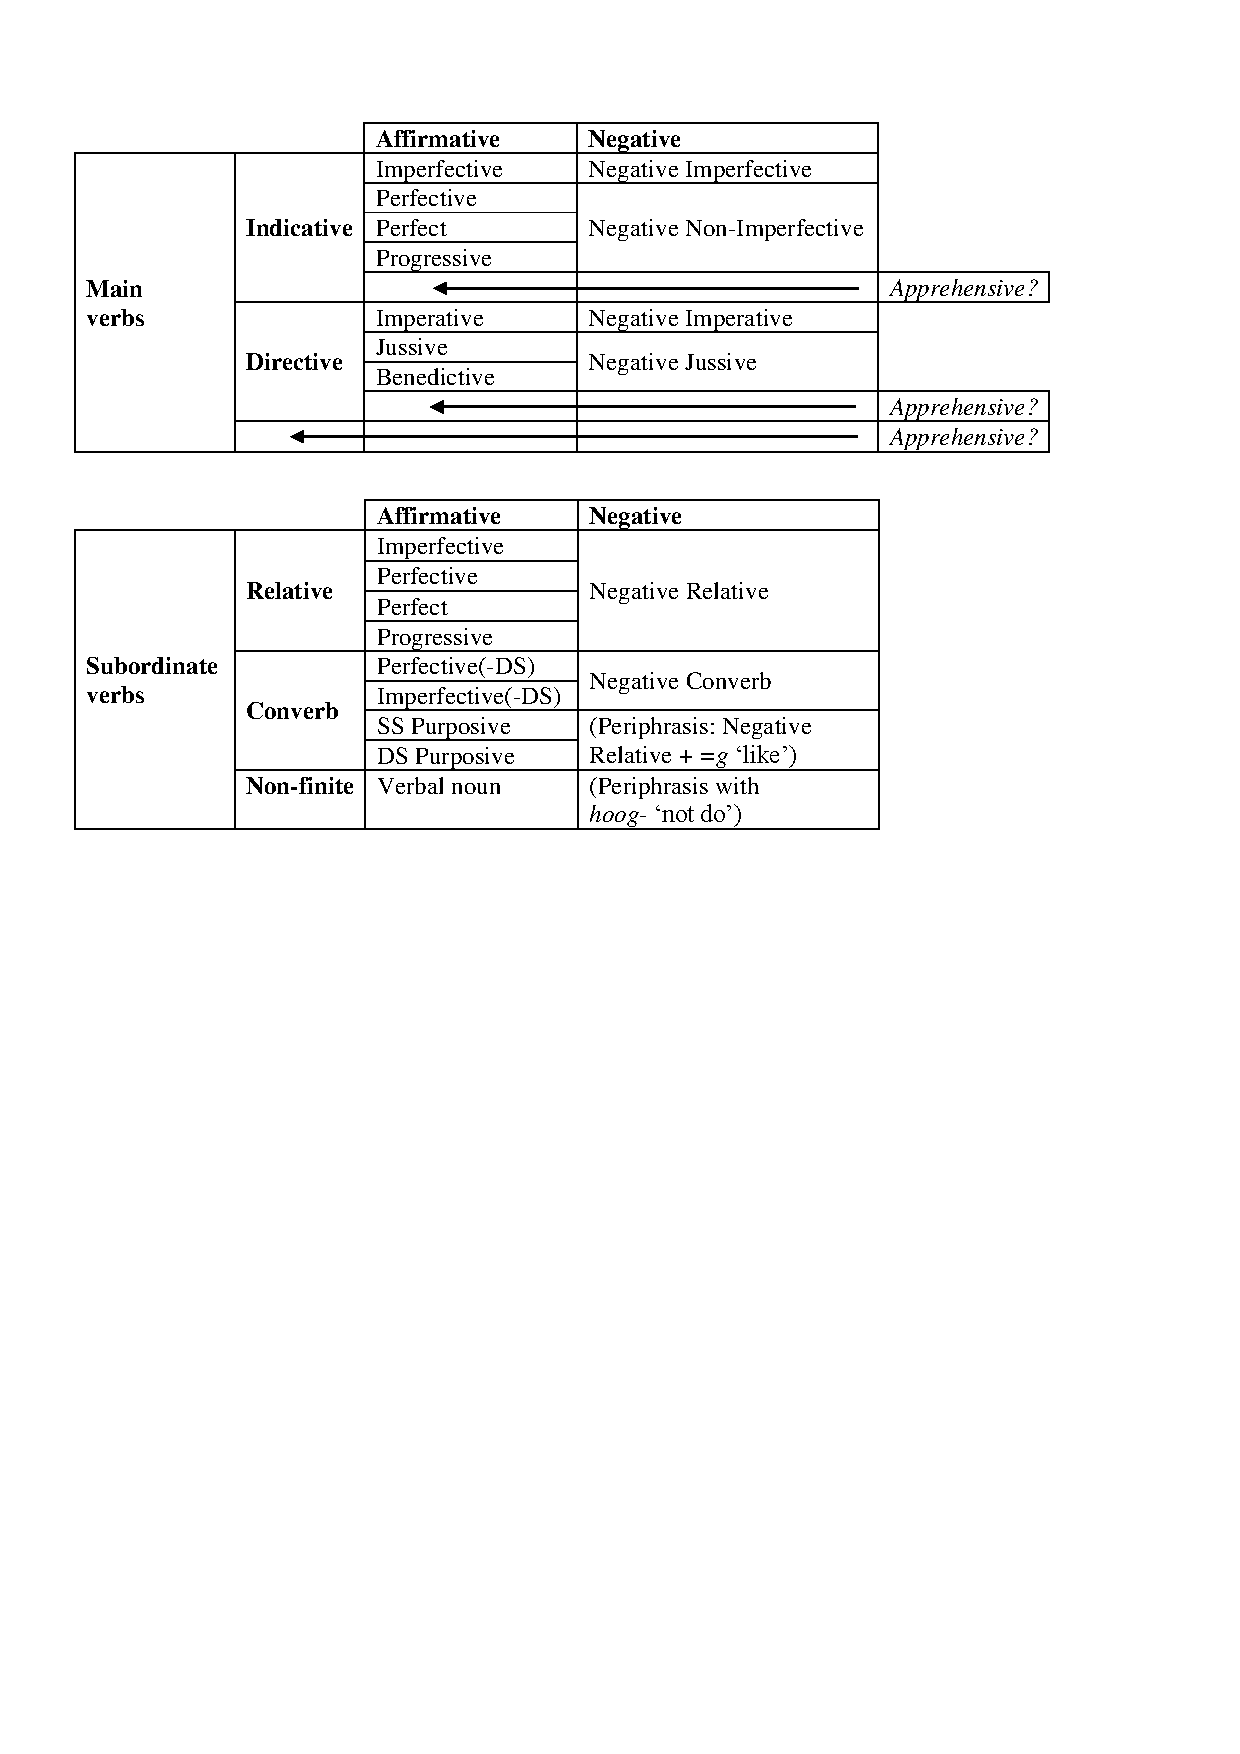
\includegraphics[width=\textwidth]{figures/Figure1.pdf}
    \caption{Classification of Kambaata verb forms}
    \label{fig:treis:1}
\end{figure}

Determining the exact place of the apprehensive in this classification is not trivial. If the criterion of morphological structure is applied, then the apprehensive clearly patterns with affirmative indicative main verbs. Like indicative verbs, it has two slots of subject morphology (\figref{fig:treis:2}), whereas directive verbs have only one subject slot (\figref{fig:treis:3}) preceding the aspect\slash mood (A/M) slot. The bipartite, discontinuous subject indexes of indicative verbs are likely the result of the fusion of a periphrastic verb form consisting of a subordinate verb and a superordinate auxiliary, each of which contributed its subject index slot to the fused verb.

\begin{figure}
    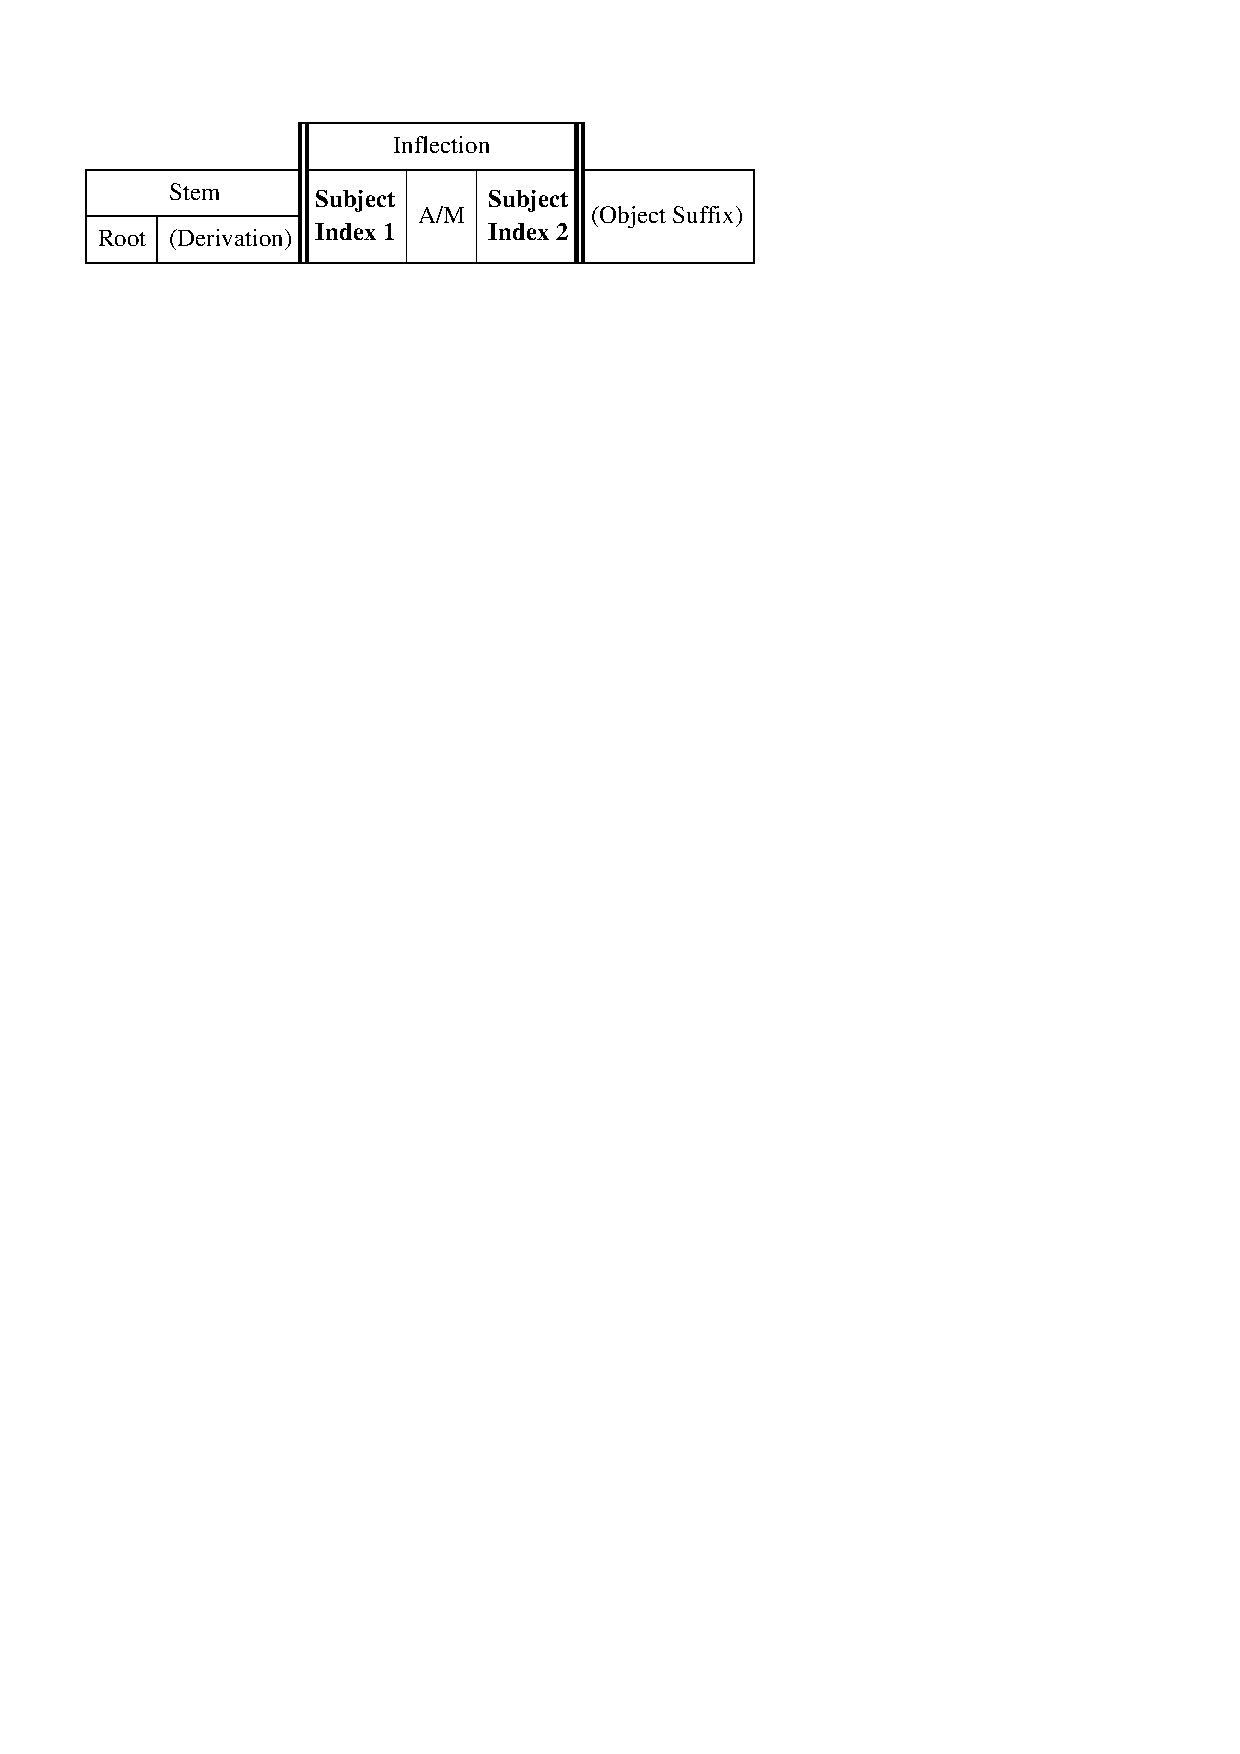
\includegraphics[width=.75\textwidth]{figures/Figure3.pdf}
    \caption{Structure of inflected verbs with two subject index slots (all affirmative indicative verbs, \textbf{apprehensive}, negative imperfective, affirmative relative)}
    \label{fig:treis:2}
\end{figure}

\begin{figure}
    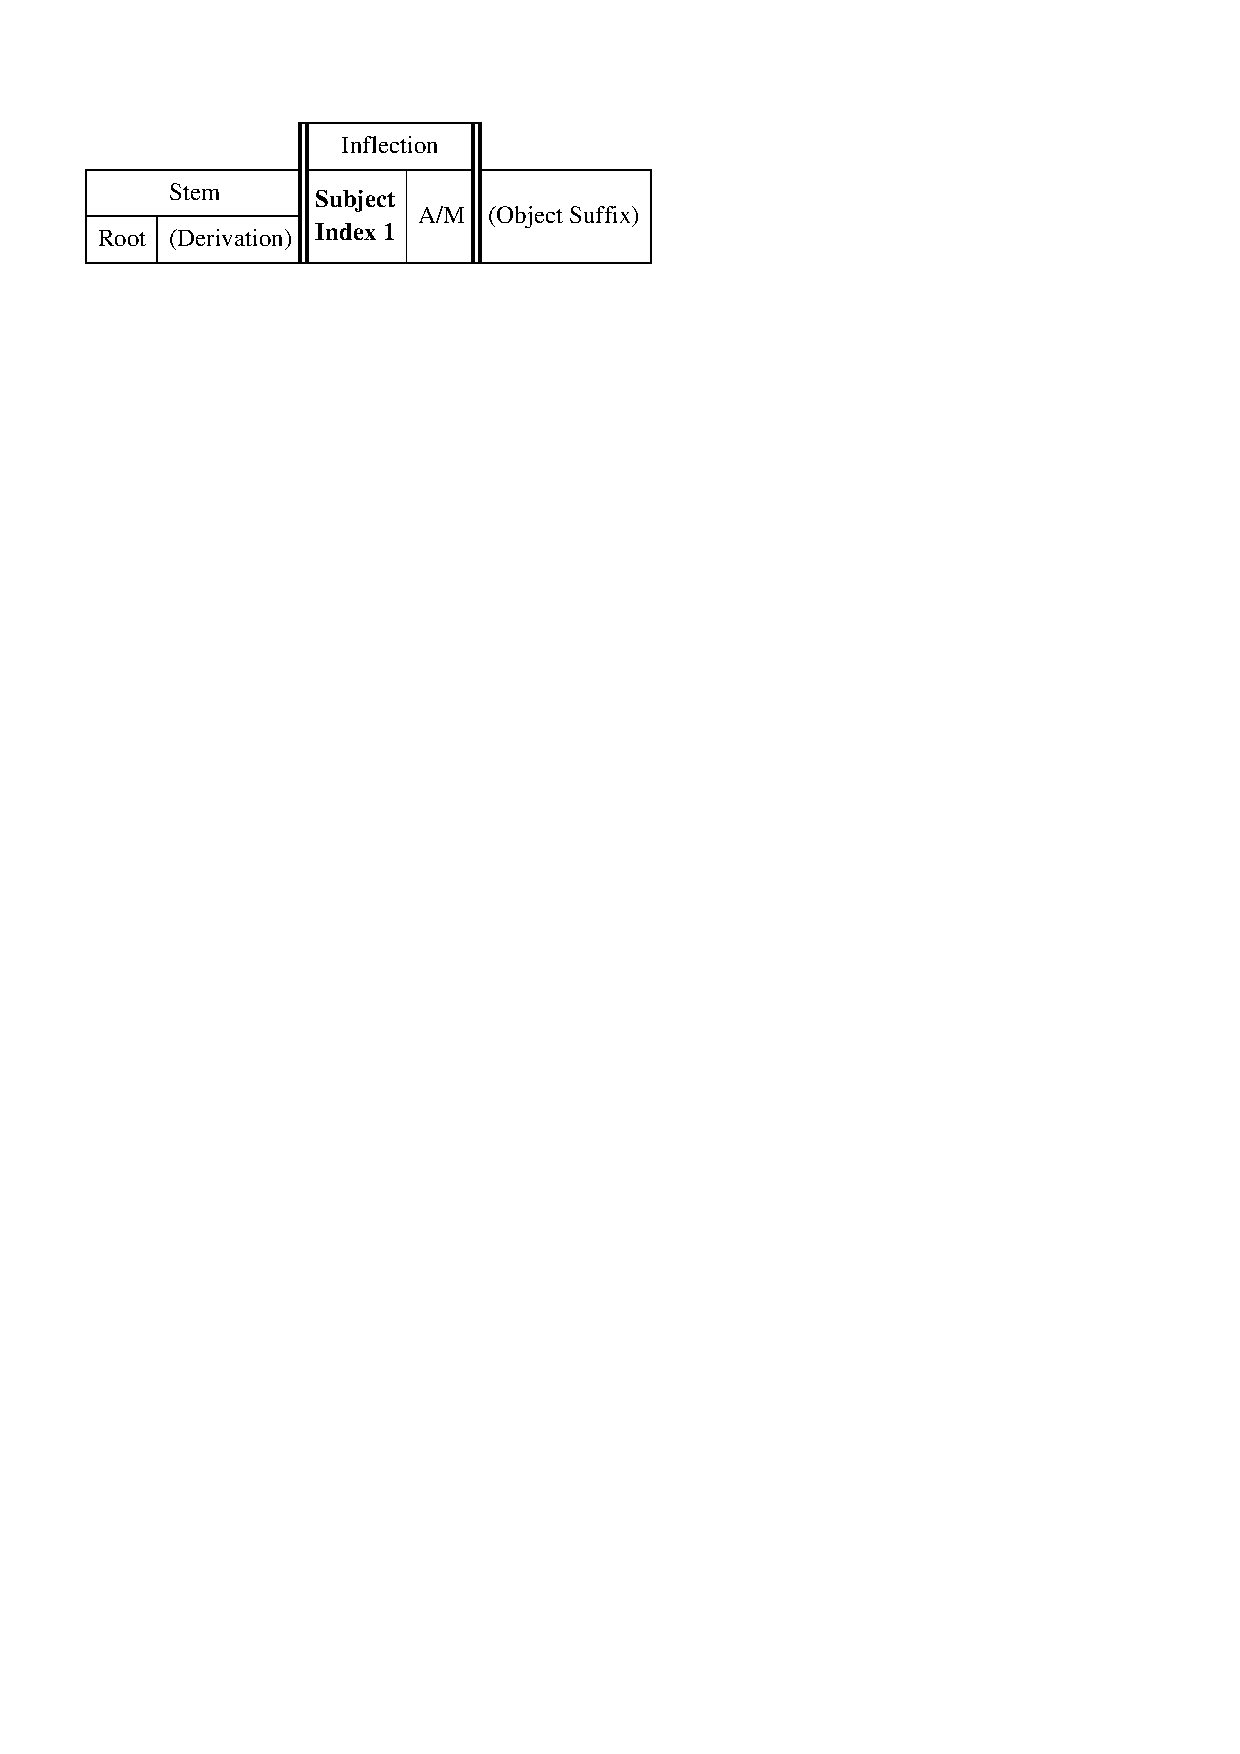
\includegraphics[width=.66\textwidth]{figures/Figure2.pdf}
    \caption{Structure of inflected verbs with one subject index slot (all affirmative and negative directive verbs, negative non-imperfective, negative relative, all affirmative and negative converbs)}
    \label{fig:treis:3}
\end{figure}

Other criteria suggest that the apprehensive is better considered to be a type of directive verb together with the imperative and the jussive. The discussion of the meaning of the apprehensive in \sectref{sec:treis:3} shows that it shares semantic features with the negative imperative and jussive. Furthermore, two formal criteria set the apprehensive apart from indicative verbs and align it with directive verbs: (i)~The apprehensive cannot be relativised, unlike all indicative verbs \citep[222--226]{Treis2012} and (ii) The apprehensive may not combine with the past and counterfactual particle \textit{íkke} -- again unlike all indicative verbs \citep{Treis2015}. Finally, the combinability of the apprehensive with pragmatically determined verbal suffixes (e.g.\ mitigators, markers of (non-)shared knowledge, speaker attitude) seems to be similar to that of directives.\footnote{The last statement is to be taken with due care as the pragmatically determined verbal suffixes, which are a characteristic trait of natural conversations, are still little investigated and would make an interesting subject for future research.} 
Finally, one may also consider establishing a third sub-category of main verb forms for the apprehensive alone -- see the third option in \figref{fig:treis:1}. Unlike all other main verbs, the apprehensive does not come in an affirmative-negative polarity pair and cannot be morphologically negated.\footnote{The use of any of the five negative morphemes the language has \citep{Treis2012Neg} is judged ungrammatical by native speakers.} Instead, (near) antonymic lexical pairs may express warnings with opposite polarity\footnote{The verb \textit{kot}- `not suffice, be (too) little', for instance, may be employed as the opposite of \textit{ih}- `suffice' and \textit{bata'}- `be (too) much'. The semantically fairly general verb \textit{fa'is}- `save, leave behind, leave out, skip, not impact' can stand in as the antonym of various verbs expressing events that causally affect a participant (e.g.\ \textit{ba'is}- `destroy, damage', \textit{sh}- `kill', \textit{woqqar}- `beat').} or speakers resort to periphrastic means to express apprehension that something may \textit{not} happen. In (\ref{ex:treis:4add}), the danger of not noticing is rendered as a danger of passing by without noticing, in which case the negation (see the morpheme \textsc{neg4}) is marked on the subordinate converb rather than on the apprehensive verb.

\ea\label{ex:treis:4add}  
\gll Háy láshsh=y-ít otá'-i! Xuu<n>du'nnáan \textbf{hi<n>gókkoomm}.\\ 
please.\textsc{intj} slow.\textsc{ideo}=say-\textsc{2sg.pfv.cvb} drive-\textsc{2sg.imp} see\textsc{<1pl>.neg4} pass\textsc{<1pl>.appr} \\
\glt `Please, drive slowly! We might pass (the sign) without noticing (it)!'  [Elicited, Field notes 2021]
\z

\subsection{The morphological structure of the apprehensive}\label{sec:treis:2.2}

The apprehensive paradigm distinguishes between seven bipartite, discontinuous subject indexes (\tabref{tab:treis:2}), of which the first element precedes and the second element follows the apprehensive morpheme \nobreakdash-\textit{ókkoo}: \textsc{1sg,} \textsc{2sg}, \textsc{3m}, \textsc{3f/3pl}, \textsc{3hon}, \textsc{1pl}, and \textsc{2pl/2hon}. The subject indexes in the first slot (\textsc{sbj1}) are identical across all finite and partially finite verb forms of \ili{Kambaata}, those in the second slot (\textsc{sbj2}) are only found in indicative affirmative main verbs and in the indicative negative imperfective paradigm.\footnote{There are slight differences in the \textsc{3m}, \textsc{3hon} and \textsc{2pl/2hon} morphemes of the \textsc{sbj2} slot across the main verb paradigms; see \tabref{tab:treis:5}.}  The apprehensive morpheme that is wedged between the two parts of the discontinuous subject marker occupies the same position as aspect morphemes (imperfective, perfective, perfect, progressive); aspect-marking and apprehensive morphology is thus mutually exclusive.\footnote{The aspect\slash mood slot in \figref{fig:treis:2} and \figref{fig:treis:3} may be filled by one morpheme only.} 

%column width needs to be adapted
\begin{table}
\fittable{\begin{tabular}{llllll}
\lsptoprule
&                  &                 &               & \multicolumn{2}{c}{Examples}\\\cmidrule(lr){5-6}
&  	-\textsc{sbj1} & -\textit{ókkoo} & \textsc{sbj2} &  \textit{ub}- `fall' & \textit{torr}- `throw'\\
\midrule
\textsc{1sg} & -∅ & -\textit{ókkoo}	& -\textit{mm}  &  \textit{ub-ókkoomm} & \textit{torr-ókkoomm}\\
\textsc{2sg} &	-\textit{t}	& -\textit{ókkoo} & -\textit{nt}  &  \textit{ub-bókkoont} & \textit{torr-i-tókkoont}\\
\textsc{3m}	& -∅ & -\textit{ókkoo}	& -\textit{'u}	 &  \textit{ub-ókkoo'u} & \textit{torr-ókkoo'u}\\
\textsc{3f/3pl} & -\textit{t} & -\textit{ókkoo} & -\textit{'u}  &  \textit{ub-bókkoo'u} & \textit{torr-i-tókkoo'u}\\
\textsc{3hon} & -\textit{een} &	-\textit{ókkoo} & -\textit{mma}  & 	\textit{ub-eenókkoomma} & 	\textit{torr-eenókkoomma}\\
\textsc{1pl} & 	-\textit{n} & -\textit{ókkoo} & -\textit{mm}  &  \textit{u<m>b-ókkoomm} & \textit{torr-i-nókkoomm}\\
\textsc{2pl/2hon} &	-\textit{t-een} & -\textit{ókkoo} & -\textit{nta}  &  \textit{ub-beenókkoonta} & \textit{torr-i-teenókkoonta}\\
\lspbottomrule
\end{tabular}}
    \caption{The apprehensive paradigm}
    \label{tab:treis:2}
\end{table}

At the boundary between the verb stem and the first subject index slot, predictable morphophonological processes are observable, as the exemplary paradigms of \textit{ub}- `fall' and \textit{torr}- `throw' in \tabref{tab:treis:2} illustrate. Assimilation, epenthesis and metathesis help prevent illicit consonant clusters when \textsc{2sg} or \textsc{3f/3pl} -\textit{t} or \textsc{1pl} \nobreakdash-\textit{n} meet C- and CC-final verb stems. In the examples given in this contribution, the discontinuous subject index and the apprehensive morpheme are not segmented from each other, but the inflectional complex (see \figref{fig:treis:2}) is glossed as if it was a portmanteau-morpheme, namely as \textsc{1sg.appr}, \textsc{2sg.appr}, etc. Predictable morphophonological changes are not indicated in the glosses either. 
Dependent object pronouns are suffixed after the second subject index slot -- see, for instance, (\ref{ex:treis:1}), (\ref{ex:treis:5}), (\ref{ex:treis:6}) and (\ref{ex:treis:19}). Pragmatically determined discourse suffixes may occur in the slot after the object pronouns -- see, for instance, (\ref{ex:treis:11}). The morphological structure of the apprehensive verb is sketched in \figref{fig:treis:4}.

\begin{figure}
% % %     \includegraphics[width=.75\textwidth]{figures/figure_treis_4corr.png}
    \begin{tikzpicture}
    \matrix [matrix of nodes, nodes={draw, font=\strut}, inner sep=1ex, column sep=-.4pt]
      {
        Root &
        (-Derivation) & 
        -\textsc{sbj}1 & 
        -\textit{ókkoo} &
        -\textsc{sbj}2 & 
        (-\textsc{obj}) & 
        (-\textsc{prag}) \\
      };
    \end{tikzpicture}
    \caption{Morphological structure of the apprehensive verb}
    \label{fig:treis:4}
\end{figure}

\section{Semantics}\label{sec:treis:3}

The discussion of the semantics of the apprehensive divides into three sections that treat third (\sectref{sec:treis:3.1}), first (\sectref{sec:treis:3.2}) and second person forms (\sectref{sec:treis:3.3}). The division of \sectref{sec:treis:3} into subsections for different persons is motivated by \citegen{vuillermet2018a} observation that languages may impose person restrictions on apprehensives, that some person forms may be less frequent than others, and/or that certain persons favour default readings.

\subsection{Third person apprehensive forms}\label{sec:treis:3.1}

In the third person, the apprehensive forms express warnings of potential events that the speaker is worried about, that they consider undesirable if not dangerous and that they expect the addressee to avert. Pre-emptive measures do not need to be expressed overtly -- but they are often mentioned in adjacent sentences or in clauses that are subordinate to the apprehensive clause (see details in \sectref{sec:treis:4}). As shown in \tabref{tab:treis:2}, \ili{Kambaata} distinguishes three third person forms: masculine, feminine\slash plural and honorific\slash impersonal.\footnote{By accident, all apprehensive forms in (near-)natural examples have \textsc{3m} subjects; \textsc{3f} and \textsc{3hon} forms are only attested in elicited data.}  In the introductory example (\ref{ex:treis:1}), a husband warns his wife of a dangerous river, which might make her drown. In (\ref{ex:treis:5}), from a recorded conversation about birth traditions, the quoted impersonal speakers (= the Kambaata people) fear that a young mother falls victim to a disease. As a pre-emptive measure, the mother leaves the house with a knife and a bunch of sooty straw in her hand. The addressees of the reported speech event are unexpressed but can be assumed to be her family members.

\ea\label{ex:treis:5}
\gll \textnormal{(\ldots)} 	shum-áa 		ful-taní-i \textnormal{(\ldots)}  billaww-ahá-a 		ka 					xit-ahá-a 			áf-f ful-táa'u, 			michch-\textbf{ókkoo}-se 						y-éeni-yan \textnormal{(\ldots)}\\
{} urine-\textsc{f.dat} go.out-\textsc{3f.ipfv.cvb-add} {} knife-\textsc{m.acc-add} \textsc{a\_dem1.m.acc}	soot-\textsc{m.acc-add}	seize-\textsc{3f.pfv.cvb} go.out-\textsc{3f.ipfv} cause.disease.sp-\textsc{3m.appr-3f.obj} say-\textsc{3hon.pfv.cvb-ds} \\
\glt (Speaking about a woman who has recently given birth) `(\ldots) and when she goes out to pee, she grabs a knife and this (bunch of straw smeared with) soot, (because one) says (among the Kambaata): ``She (as a young mother) might get attacked by the \textit{michcha}-disease''.'  (lit. `it might \textit{michcha} her') [Recorded conversation, EK2016-02-23\_002]
\z

Also the following apprehensive examples from the written corpus are found in direct speech reports. Example (\ref{ex:treis:6}) is a self-quotation, in which the speaker reports a warning from an internal monologue.\footnote{I refer here to the form \textit{kar-ókkoo-he}; second person forms such as \textit{waal-tókkoont} and their prohibitive pragmatic force are discussed in \sectref{sec:treis:3.3}.} Example (\ref{ex:treis:7}) is here presented to demonstrate that the quoted speaker (and not the actual speaker\slash writer) is the source of the evaluation of the situation as undesirable and as apprehension-causing.\footnote{All examples taken from publications in the \ili{Kambaata} language are stress-marked, segmented, glossed and translated to English by the present author.}

\ea\label{ex:treis:6} 
\gll \textnormal{(\ldots)} án waal-tókkoont y-áayyoommi-i worr-íichch-u kar-\textbf{ókkoo}-he y-í-ne-eb-be.\\
{} \textsc{1sg.nom}	come-\textsc{2sg.appr}	say-\textsc{1sg.prog.rel-nmlz1.m.nom} snakes-\textsc{sgv-m.nom} sting-\textsc{3m.appr-2sg.obj} say-\textsc{1sg.pfv.cvb-l-cop3-prag5}\\
\glt (Little Prince speaking to the pilot) `(\ldots) I said ``(Better) you don't come!'' (because) I thought (lit. `said') ``The snake might bite you''.' \citep[87]{Saint-Exupéry2018}
\z 

\ea\label{ex:treis:7} 
\gll Gag-á-s						sh-eenáni-yan		``Arg-é			oddishsh-áta qég-u				ba'-is-\textbf{ókkoo'u}'' 						y-ée'u. \\
self-\textsc{m.acc-3m.poss} kill-\textsc{3hon.ipfv.cvb-ds} \hphantom{[}loan-\textsc{f.gen} clothes-\textsc{f.acc}
blood-\textsc{m.nom} become.spoilt-\textsc{caus1-3m.appr} say-\textsc{3m.pfv}\\
\glt (Proverb) `When he is being killed, he says, ``The blood might spoil the borrowed clothes.''' (i.e.\ `He is more worried about his borrowed clothes than his own life.') \citep[52]{AlamuAlamaayyo2017}
\z

\ili{Kambaata} does not seem to impose any semantic restrictions on the verbs that can serve as input for the apprehensive form. One finds, for instance, also inchoative-stative property verbs in warnings (\ref{ex:treis:8}).

\ea\label{ex:treis:8}
\gll Juus-áan		hoolam-á 		wo'-á 			wór-tooti, 				qac-\textbf{ókkoo'u}. \\
juice-\textsc{m.loc}	much-\textsc{m.acc}	water-\textsc{m.acc}	put.in-\textsc{2sg.imp.neg2}	become.thin-\textsc{3m.appr}\\
\glt `Don't pour too much water into the juice, it might become (too) thin.'  [Elicited, Field notes 2019]
\z 

Furthermore, \ili{Kambaata} does not exclude verbs that typically express positive states of affairs, such as \textit{bajig}- `be(come) happy', from apprehensive clauses. However, when such verbs are apprehensive-marked, the event is evaluated as negative for the speaker and/or the addressee. In (\ref{ex:treis:9}), the speaker is worried that the addressee's enemy is happy about the addressee's failure.

\ea\label{ex:treis:9}
\gll Qáar-t						huját-i! 			Bux-xoontí=da						díin-u bajig-\textbf{ókkoo'u}. \\
become.strong-\textsc{2sg.pfv.cvb}	work-\textsc{2sg.imp}	become.poor-\textsc{2sg.pfv.rel=cond} enemy-\textsc{m.nom} become.happy-\textsc{3m.appr}\\
\glt `Work hard! If you sink into poverty, the enemies might be happy.'  [Elicited, Field notes 2019]
\z 

\subsection{First person apprehensive forms}\label{sec:treis:3.2}

First person singular and plural apprehensive forms are the least frequent forms in my corpus (see \tabref{tab:treis:1}), hence I supplemented the two examples from the schoolbooks, which are quoted in (\ref{ex:treis:13}) and (\ref{ex:treis:16}), by elicited sentences and invented dialogues. In the first person, as in the third person (\sectref{sec:treis:3.1}), the apprehensive is used to utter warnings of looming dangers and potential accidental events, such as a dangerous fall (\ref{ex:treis:10}), an unintended breach of social conventions (\ref{ex:treis:11}), or a car crash (\ref{ex:treis:13}). The speaker assumes the addressee to be able to take pre-emptive steps in order to avert the undesirable event.

\ea\label{ex:treis:10} 
\gll Ub-\textbf{ókkoomm}, 	ka 					masalaal-á 	áf-i! \\
fall-\textsc{1sg.appr}		\textsc{a\_dem1.m.acc}	ladder-\textsc{m.acc}	seize-\textsc{2sg.imp}\\
\glt (Possible context provided: Speaker is standing on a ladder that is held by the addressee) `(Take care!) I might fall. Hold the ladder!'  [Elicited, Field notes 2019]
\z 

\ea\label{ex:treis:11} 
\gll Osa'll-\textbf{ókkoom}-be, 	sá! \\
laugh-\textsc{1sg.appr-prag5} shush.\textsc{intj}\\
\glt (Context: On the way to visit a mourning family, Speaker\textsubscript{i} asks Addressee\textsubscript{j} to keep his\textsubscript{j} mouth shut so that he\textsubscript{i} wouldn't burst out laughing. However, Addressee keeps chatting away. Speaker interrupts him:) `(Watch out!) I might laugh (as I said earlier), shush!' [Mock dialogue, DW2019-02-17]\\
\z 

The worried speaker and the alerted addressee can be the same person, as in (\ref{ex:treis:12}), which is a warning to self.

\ea\label{ex:treis:12} 
\gll Ub-\textbf{ókkoomm}, 	qoraphph-eemmí=da 					xúm-a-a. \\
fall-\textsc{1sg.appr}	take.care.\textsc{mid-1sg.pfv.rel=cond}	good-\textsc{m.pred-m.cop2}\\
\glt (Possible context provided: Speaker spots a slippery spot ahead of them and tells themself) `I might fall, it's good to be careful.'  [Elicited, Field notes 2003, 2019]
\z 

The potential event is undesirable for the speaker (\ref{ex:treis:10})--(\ref{ex:treis:12}), or the speaker and their group (\ref{ex:treis:13}).

\ea\label{ex:treis:13} 
\gll Háy 			láshsh=y-ít 				otá'-i! 			Ka'llixx-áan 		\textbf{aa<n>gókkoomm}. \\
please.\textsc{intj} slow.\textsc{ideo}=say-\textsc{2sg.pfv.cvb}	drive-\textsc{2sg.imp}	accident-\textsc{m.loc}	enter\textsc{<1pl>.appr}\\
\glt (Speaker warns a speeding driver) `Please, drive slowly! We might have (lit. `enter') an accident.' \citep[4.55]{KEB2008a}
\z 

Apart from expressing the speaker's fear of an undesirable event with a negative impact on themself, the first person apprehensive form is also used for threats. Here the potential danger is not accidental but inflicted on the addressee by the speaker. The event expressed in the apprehensive clause can be straightforwardly undesirable for the addressee, such as the kicks in (\ref{ex:treis:14}) and the speaker's betrayal of a secret in (\ref{ex:treis:15}), or have undesirable consequences, such as the inevitable punishment that would follow if the speaker saw the addressee breaking the rules in (\ref{ex:treis:16}).

\ea\label{ex:treis:14} 
\gll Ool-\textbf{ókkoon}-ke! \\
kick-\textsc{1sg.appr-2sg.obj}\\
\glt (Possible context provided: Addressee has been teasing Speaker for a while; Speaker threatens) `(Stop it, otherwise) I kick you!' [Elicited, Field notes 2019]
\z 

\ea\label{ex:treis:15} 
\gll Mát-o 		bar-e-'ée=bii 					kul-\textbf{ókkoomm}. \\
one-\textsc{m.obl}	day-?-\textsc{assoc.f.gen=nmlz2.m.acc} tell-\textsc{1sg.appr}\\
\glt (Possible context provided: Speaker knows a secret of Addressee that they promised to keep. Now that Addressee annoys them, they threaten) `(Stop it, otherwise) I might tell/reveal that (secret) of the other day!'  [Elicited, Field notes 2004]
\z 

\ea\label{ex:treis:16} 
\gll Íi			béet-o,		lankíi	kánn					haqq-í			al-í ful-táni-yan			xuud-\textbf{ókkoon}-ke. \\
\textsc{1sg.gen} son-\textsc{m.voc}	again	\textsc{a\_dem1.m.obl}	tree-\textsc{m.gen}	top-\textsc{m.acc} go.up-\textsc{2sg.ipfv.cvb-ds} see-\textsc{1sg.appr-2sg.obj}\\
\glt (Context: Although the mother has strictly forbidden it, a boy (= the addressee) keeps on climbing onto the tree in the front yard. The mother gets angry and threatens him) `(Stop it,) my son, I might see you climbing this tree again (and this will have negative consequences)!'  \citep[4.45]{KEB1989}
\z

\citet{vuillermet2018a} shows in her cross-linguistic study of 46 South American and Australian languages that only 63.6\% of the languages with apprehensive morphology have first person forms attested. Of the 17 languages that have first person transitive subject forms of [+control] verbs, one language, \ili{Matsés}, permits only a warning reading but excludes a threat reading in the first person. For the other 16 languages, the apprehensive forms are found in threats or both in threats and warnings. \ili{Kambaata}, like  e.g.\ \ili{Ese Ejja} \citep[273--274]{vuillermet2018a}, does not impose a warning or threat reading with [+control] in the first person, as the two possible translations of the `hit'-verb in (\ref{ex:treis:17}) show.

\ea\label{ex:treis:17} 
\gll Woqqar-\textbf{ókkoon}-ke! \\
hit-\textsc{1sg.appr-2sg.obj}\\
\glt (i)	(Threat) `(Stop it, or) I  hit you!' \newline
(ii)	(Warning) `(Watch out! Step aside, otherwise) I might accidentally hit you!' (Deginet Wotango Doyiso, personal communication, 2020)
\z

\subsection{Second person apprehensive forms}\label{sec:treis:3.3}

The second person apprehensive forms are not only the most frequently attested forms in the database (\tabref{tab:treis:1}) but also commonly overheard in conversations. In (\ref{ex:treis:18}), the speaker expresses concern that the addressee might finish the coffee to his (= the addressee's) disadvantage. In (\ref{ex:treis:19}), the speaker is worried about a potential infection. In an example from oral literature in (\ref{ex:treis:2}), a girl warns a boy about the potential undesirable consequences of his advances. The looming, dangerous or disadvantageous situation is undesirable for the speaker and/or the addressee -- or to phrase it more generally, apprehensives express events that can be evaluated negatively by any discourse participant.

\ea\label{ex:treis:18} \textnormal{Overheard in a \ili{Kambaata} household (2019)}\\
\gll Kesáa	xoof-\textbf{fókkoont}. \\
\textsc{2sg.dat} finish-\textsc{2sg.appr}\\
\glt (Observed context: Addressee has boiled coffee for three people, now he is generously filling two cups for Speaker and a third person. Speaker is worried that not enough will be left in the pot to also fill Addressee's own cup.) `(Take care!) You might finish it to your disadvantage!'\slash `Don't finish it off on yourself!'\\
\z 

\ea\label{ex:treis:19} 
\gll Gansh-ú-kk 			hig-is-\textbf{sókkonte}-'e, shiin-á-kk 				waal-áam-ba'a. \\ 
cold-\textsc{m.acc-2sg.poss} pass-\textsc{caus1-2sg.appr-1sg.obj} side-\textsc{m.acc-2sg.poss} 	come-\textsc{1sg.ipfv-neg1}\\
\glt `You might pass on the cold to me, I won't be coming near you.' [Elicited, Field notes 2019]
\z 

 The two alternative translations in (\ref{ex:treis:2}) and (\ref{ex:treis:18}) reflect the recurring difficulty to decide whether second person apprehensive forms are better translated as warnings of a worried speaker or as simple negative commands. The use of the conative interjection \textit{háy} `please, I beg you' with the apprehensive form in (\ref{ex:treis:20}) shows that the utterance is possibly less a warning of an imprudent, unintentional realisation of an event (`you might hurry on') than a request (`do not hurry on').

\ea\label{ex:treis:20} 
\gll Ta	ma'nn-ichch-ú<n>ta-ma	iill-iteentáachch háy			sarb-an-\textbf{teenókkoonta}. \\
\textsc{a\_dem1.f.acc} place-\textsc{sgv-f.acc<emp>-cf}	reach-\textsc{2pl.pfv.rel.abl} please.\textsc{intj}	hurry-\textsc{pass-2pl.appr}\\
\glt (Pilot to the readers of the Little Prince:) `If you should come upon this very spot, please, do not hurry on.' \citep[95]{Saint-Exupéry2018}
\z 

 In contexts such as (\ref{ex:treis:20}), the semantic differences between second person apprehensive and negative imperative forms (singular: ´-\textit{tooti}, plural: \nobreakdash-\textit{téenoochche}) are subtle and hard to pinpoint, and native speakers often accept a swap of the apprehensive for regular negative imperative forms and vice versa. In discussions about the meaning differences, speakers voice conflicting intuitions. The verb forms are sometimes qualified as synonymous, or the apprehensive is interpreted as a reinforced (\ref{ex:treis:21}), occasionally even as a mitigated command (\ref{ex:treis:20}). It seems safe to assume that mitigation and reinforcement are not inherent to the second person apprehensive forms but contributed by other elements in the linguistic context, such as the polite interjection in (\ref{ex:treis:20}), the adverb \textit{hináten} `by any means, at all' in (\ref{ex:treis:21}) and possibly various other factors. 

\ea\label{ex:treis:21} 
\gll Buchch-á ít-i!	\textnormal{[Definition:]} mat-ú íkk-ee xaw-á huj-íta hinát-e-n agur-\textbf{tókkoont} y-éen qaar-s-íi		y-eennó yann-á. \\
soil-\textsc{m.acc} eat-\textsc{2sg.imp} {} one-\textsc{m.acc}	become-\textsc{3m.prf.rel}	issue-\textsc{m.acc} work-\textsc{f.acc} totality-\textsc{f.obl-emp}	abandon-\textsc{2sg.appr}		say-\textsc{3hon.pfv.cvb} become.strong-\textsc{caus1-m.dat}	say-\textsc{3hon.ipfv.rel} saying-\textsc{m.acc}\\
\glt (Dictionary entry) `Eat soil! (i.e.\  Persevere!)' = (Definition) `Saying that is uttered to encourage (lit. `strengthen') (somebody), meaning ``Do not, by any means, give up on a problem (or) a job!''' \citep[158]{Alemu2016}
\z 

The near synonymy of the apprehensive and the negative imperative is also reflected in the written \ili{Kambaata} literature where the two verb forms may occur in identical contexts; see the Bible excerpt in (\ref{ex:treis:22}).

\ea\label{ex:treis:22}
\gll Bookk-íta 	it-\textbf{téenoochche}; \textnormal{(\ldots)} 	resh-á-ssa-n 						ul-\textbf{teenókkoonta}. \\
pigs-\textsc{f.acc}	eat-\textsc{2pl.imp.neg2} {} carcass-\textsc{m.acc-3pl.poss-emp}	touch-\textsc{2pl.appr}\\
\glt (Deuteronomy 14,8) `Don't eat pigs; (\ldots) don't touch their carcasses.'   \citep{KHTPHNodate}
\z 

Despite examples such as (\ref{ex:treis:21}) and (\ref{ex:treis:22}),\footnote{See also the second person apprehensive form used for the prohibition of a willful action in (\ref{ex:treis:6}).} the apprehensive tends to express warnings of unintended, undesirable actions and the negative imperative prohibitions of actions that the addressee carries out wilfully, as can also be seen in ``minimal pairs'' such as (\ref{ex:treis:23}) and (\ref{ex:treis:24}). All speakers I consulted agreed that (\ref{ex:treis:23}) is a warning of an unintentional step into the mud, while (\ref{ex:treis:24}) is a prohibition of an intentional step into the mud. Similarly, the imperative \textit{úb-booti} (fall-\textsc{2sg.imp.neg2}) `don't fall' is only considered felicitous when the addressee is intentionally falling down, e.g. to practice it, and the speaker wants them to stop, while \textit{ub-bókkoont} (fall-\textsc{2sg.appr}) `(watch out!) don't fall' is used as a warning of an unintended fall.

\ea\label{ex:treis:23}
\gll Orc-áan aag-\textbf{gókkoont}. \\
mud-\textsc{m.loc} enter-\textsc{2sg.appr}\\
\glt (Possible context provided: Addressee approaches a muddy spot. Speaker warns Addressee of a danger) `(Watch out!) You might step into the mud!'\slash `Don't step (accidentally) into the mud!'  [Elicited, Field notes 2005]
\z 

\ea\label{ex:treis:24} 
\gll Orc-áan áag-\textbf{gooti}!\\
mud-\textsc{m.loc} enter-\textsc{2sg.imp.neg2}\\
\glt (Possible context provided: Addressee,  e.g.\ a child, is happily jumping into every mud pit on the way) `Don't step (intentionally) into the mud!'  [Elicited, Field notes 2005]
\z 

\citet{Dobrushina2006} and \citet{pakendorfschalley2007} have documented a grammaticalization path from markers of possibility to prohibitives via intermediate stages of apprehension and warning. \ili{Kambaata} gives further evidence for this diachronic development. The apprehensive verb form, which is used to express the speaker's concern about the realisation of an undesirable potential event, as is still clearly seen in the first (\sectref{sec:treis:3.2}) and third persons (\sectref{sec:treis:3.1}), becomes more and more interpreted as a prohibitive in the second persons. The pre-emptive measure originally only implicit in the apprehensive verb (or expressed in adjacent clauses) has become its central meaning component, whereas the apprehensional component is backgrounded or lost: `You might finish it' (implicit: `Take care not to'). > `Do not finish it!' However, the existence of contexts such as (\ref{ex:treis:23}) and (\ref{ex:treis:24}) where either only second person negative imperative or second person apprehensive forms are felicitous shows that the verb forms are not yet fully synonymous.

\section{Syntax}\label{sec:treis:4}

The verbal paradigms of \ili{Kambaata} split up into those used in main clauses and those used in subordinate clauses (\figref{fig:treis:1}); main clause verbs can constitute a complete sentence on their own. Apprehensive verbs are main clause verbs and, due to \ili{Kambaata}'s fairly strict head-finality, they usually occur sentence-finally (cf.\  \sectref{sec:treis:1.2} and \sectref{sec:treis:2.1}). It is only in reported speech constructions that we find apprehensive verbs in a sentence-medial position, see (\ref{ex:treis:5})--(\ref{ex:treis:7}) and (\ref{ex:treis:21}).\footnote{Another exception to the head-finality rule are examples in which constituents follow the main verb as an afterthought.} Apprehensive verbs may head complex sentences consisting of several clauses. While the apprehensive main clause -- the final clause -- expresses the apprehension-causing situation, dependent subordinate clauses -- non-final clauses -- express the temporal context or the condition under which the apprehension-causing situation is realised. It is fairly common to find the pre-emptive action expressed in a negative subordinate clause, either a converb or a conditional clause (`if not [pre-emptive action]').
Example (\ref{ex:treis:25}) consists of three clauses, of which clause 3, the main clause, contains the apprehension-causing situation, namely the subject's burning; clause 2 expresses an event that precedes the burning in time; clause 1 states the condition under which the apprehension-causing situation becomes true, namely under the condition that the addressee fails to carry out the pre-emptive action.\footnote{While it is clear that clause 1 and 2 are dependent on clause 3, the main clause, I am unable to say whether clause 1 is dependent on clause 2 or whether the two clauses are on the same level.} The subordinate clauses 1 and 2 in (\ref{ex:treis:25}) are headed by perfective converbs (\textsc{pfv.cvb}), which leave the semantic relation with the subsequent clause vague. Here the perfective converbs are interpreted as expressing a condition (\textit{hóoggiyan}) and a relation of anteriority (\textit{aphphítiyan}). 

\ea\label{ex:treis:25} 
\gll {\ob}Giir-áta  	danáam-o=gg-a 			tú'mm=a'-ú hóog-gi-yan{\cb}\textsubscript{\textnormal{\textsc{clause 1}}}		{\ob}mát-oa=rr-áan				aphph-íti-yan{\cb}\textsubscript{\textnormal{\textsc{clause 2}}} {\ob}\textbf{bu<m>bókkoomm}.{\cb}\textsubscript{\textnormal{\textsc{clause 3}}}\\
\hphantom{[}fire-\textsc{f.acc}	good-\textsc{m.obl=sim-m.obl}	narrow.down.\textsc{ideo}=do-\textsc{m.acc} not.do-\textsc{2sg.pfv.cvb-ds} \hphantom{[}one-\textsc{m.obl=nmlz4-m.loc} seize.\textsc{mid-3f.pfv.cvb-ds} \hphantom{[}burn\textsc{<1pl>.appr}\\
\glt `(Watch out!) If you don't narrow down the fire properly (to the small spot in the centre of the fireplace), it (lit. `she' = the fire) might light something, and we might burn.'  [Elicited, Field notes 2004]
\z 

In (\ref{ex:treis:26}), the pre-emptive action is expressed in a different type of subordinate clause, in a negative conditional\slash temporal clause (formally a headless, ablative-marked participial clause).

\ea\label{ex:treis:26} 
\gll Rubbat-aan-ch-ú 				áf-f 				waal-tumb-óochch gizz-á 			kam-\textbf{ókkoon}-ke. \\
guarantee-\textsc{ag-sgv-m.acc}	take-\textsc{2sg.pfv.cvb} come-\textsc{2sg.neg5-abl} money-\textsc{m.acc}	deny-\textsc{1sg.appr-2sg.obj}\\
\glt `If you don't come with a guarantor, then, (I am afraid,) I might deny you the money (i.e.\ the loan).'   [Elicited, Field notes 2004]
\z 

Most frequently, however, we find the pre-emptive action expressed in a sentence adjacent to (i.e.\ syntactically independent of) the sentence expressing the apprehension-causing situation. A typical example is given in (\ref{ex:treis:27}): here a following imperative sentence tells the addressee how to avert the danger.

\ea\label{ex:treis:27} 
\gll Tees-ó		antabee'-ú			súl-u						oróoshsh kam-\textbf{ókkoo'u}, 					háy			xúud-i! \\
now-\textsc{f.gen}	chicken-\textsc{m.acc}	predator.sp-\textsc{m.nom}	go.out.\textsc{caus1.3m.pfv.cvb} do.completely-\textsc{3m.appr}	please.\textsc{intj}	look-\textsc{2sg.imp}\\
\glt `A \textit{sula}-predator (\textit{genetta abyssinica}) might snatch these chickens away, please, look (after them)!' [Mock dialogue, DW2016-04-01]
\z 

In much the same way as in (\ref{ex:treis:27}), pre-emptive situations are expressed in syntactically independent imperative, prohibitive and indicative sentences in other examples of this chapter; see \tabref{tab:treis:3} for links to the relevant examples.

\begin{table}

    \begin{tabular}{ll}
    \lsptoprule
Preceding indicative sentence &	(\ref{ex:treis:5})\\
Following indicative sentence &	(\ref{ex:treis:12}), (\ref{ex:treis:19})\\
Preceding imperative sentence &	(\ref{ex:treis:8}), (\ref{ex:treis:9}), (\ref{ex:treis:13})\\
Following imperative sentence &	(\ref{ex:treis:10}), (\ref{ex:treis:27})\\
Following imperative interjection &	(\ref{ex:treis:11})\\
Preceding prohibitive sentence & (\ref{ex:treis:6})\\
\lspbottomrule
    \end{tabular}
    \caption{The expression of pre-emptive situations in independent sentences}
    \label{tab:treis:3}
\end{table}

It is important to note that the \ili{Kambaata} apprehensive is only found in main clauses but used neither in negative purpose clauses nor for direct embedding under `fear' predicates, unlike apprehensives in other languages that the literature reports on (cf.\  \citealt{lichtenberk1995}). Instead, as the following excursus shows, `fear' predicates in \ili{Kambaata} govern reported speech constructions. Either a direct speech report, as in (\ref{ex:treis:28a}), or an indirect speech report, as in (\ref{ex:treis:28b}), followed by the quotative verb \textit{y-} `say', is dependent on the `fear' predicate. 

\ea\label{ex:treis:28a} 
\gll \textnormal{(\ldots)} {\ob}haqq-i-sí al-íichch úbb biix-am-áno{\cb}\textsubscript{\textnormal{\textsc{direct report}}} y-éen abb-is-éen waajj-éemma. \\
{} \hphantom{[}tree-\textsc{m.gen-def} top-\textsc{m.abl} fall.\textsc{3m.pfv.cvb} break-\textsc{pass-3m.ipfv} say-\textsc{3hon.pfv.cvb} become.big-\textsc{caus1-3hon.pfv.cvb} fear-\textsc{3hon.pfv}\\
\glt `(\ldots) she (\textsc{hon}) was very afraid that he might fall down from the tree and break (a limb).' (lit. `{``}He will fall \ldots,'' (she) having said, she was very afraid.')  \citep[4.45]{KEB1989}
\z

The indirect speech construction specific to `fear' predicates consists of a quote which is marked like a negative purpose clause and which is followed by a quotative verb (\ref{ex:treis:28b}). Negative purpose clauses are negative relative clauses headed by the similative morpheme =\textit{g} `like; manner',  i.e.\ `so that the \textsc{subject} does not \textsc{verb}' is expressed as `like the \textsc{subject} does not \textsc{verb}' (see \citealt{Treis2010} and \citeyear{Treis2017} for details). Thus while the direct quote in (\ref{ex:treis:28a}) ends in a main verb form and could in principle correspond to the original statement made by the fearful subject, the indirect quote in (\ref{ex:treis:28b}) takes a subordinate (relative) form that cannot constitute an independent utterance.

\ea\label{ex:treis:28b} 
\gll J-eechch-ú-s {\ob}makíin-u fushsh-aqq-úmbo-nne=g-a{\cb}\textsubscript{\textnormal{\textsc{indir. report}}} y-ín báa<m>beemm íkke. \\
time-\textsc{sgv-f.acc-def} \hphantom{[}car-\textsc{m.nom} go.out.\textsc{caus1-mid-3m.neg5-1pl.obj.rel=sim-m.obl} say-\textsc{1pl.pfv.cvb} fear\textsc{<1pl>.prf} \textsc{pst}\\
\glt `At the time we were afraid that the bus might leave without us.' (lit. `So that the bus does not leave on us, (we) saying, we were afraid'). [Elicited, Field notes 2021]
\z 

\section{Historical origin}\label{sec:treis:5}

The \ili{Kambaata} apprehensive must have been grammaticalised fairly recently, because -- to the best of my knowledge -- no similar paradigm is found in other \ili{Cushitic} languages. Not even the grammars of the most closely related languages, \ili{Alaaba} \citep{Schneider-Blum2007}, K'abeena \citep{Crass2005}, \ili{Hadiyya} \citep{Tadesse2015} and \ili{Sidaama} \citep{Kawachi2007,Anbessa2014}, mention a verbal paradigm of similar form or function.\footnote{Even if it seems unlikely, I can, of course, not exclude that the apprehensive paradigms escaped the attention of \ili{Cushitic} grammaticographers. I could not find examples expressing warnings or threats in the grammars of any closely related language to investigate possible alternative means of expressing apprehension.} The discussion of the origin of the \ili{Kambaata} apprehensive paradigm can thus not be based on comparative but only on language-internal evidence.

I argue in this section that the apprehensive paradigm is of phrasal origin and the result of the merger of a complex verb form consisting of a same subject affirmative purposive converb\footnote{\ili{Kambaata} makes a distinction between same subject and different subject affirmative purposives (\figref{fig:treis:1}); see \citet{Treis2010} for details.} plus the existential copula \textit{yoo-} `exist, be (located)'~-- both verb forms still exist independently in the language. The diachronic development of the apprehensive is likely to have proceeded in the scenario sketched in \figref{fig:treis:5}, with Stage 4 representing the synchronic stage.

\begin{figure}[ht]
\small%
\begin{tabular}{lll}
(1) & Purposive converb + existential copula & `[\textsc{sbj}] is about to \textsc{verb}'\\
& \{Verbal stem\}-\textsc{sbj1}-\textit{ó-ka} + \textit{yóo}-\textsc{sbj2} &\phantom{a}\\
(2) & \{Verbal stem\}-\textsc{sbj1}-\textit{ó-k} + \textit{yóo}-\textsc{sbj2} & \phantom{a}\\
(3) & \{Verbal stem\}-\textsc{sbj1}-\textit{ó-k}(-)\textit{koo}-\textsc{sbj2}&\phantom{a}\\
(4) & \{Verbal stem\}-\textsc{sbj1}-\textit{ókoo}-\textsc{sbj2} & `[\textsc{sbj}] might \textsc{verb} (= undesirable)'\\ 
\end{tabular}\caption{The four stages of the apprehensive paradigm}
\label{fig:treis:5}\end{figure}
%\begin{figure}
 %   \includegraphics[width=1\textwidth]{figures/figure_treis_5_corr.png}
  %  \caption{The diachronic origin of the apprehensive paradigm}
   % \label{fig:treis:5}
%\end{figure}

At Stage 1, the purposive converb and the copula were independent words forming a complex predicate. At Stage 2, the tight syntactic link between the two words led to phonological reductions. First, the unstressed final vowel (\textit{a}) of the converb was dropped, then the resulting illicit consonant cluster simplified. The initial consonant (\textit{y}) of the copula assimilated to the abutting final consonant (\textit{k}) of the converb.\footnote{Progressive (perseveratory) place and manner assimilation processes are observed elsewhere in the language, both synchronically and historically \citep[65, 71]{Treis2008}.} Thus, at Stage 3, the periphrastic verb became interpreted as a single word, and the stress on the copula was lost. In the synchronic Stage 4, there is no longer any indication of a morpheme boundary between the converb and the copula.

In the following, I present evidence for the plausibility of the diachronic scenario in \figref{fig:treis:5}. First, I show that the existential copula is likely to have contributed the second syllable of today's apprehensive morpheme (\textit{koo}) and the second subject index slot (\textsc{sbj2}). Then, I argue that the first subject index slot (\textsc{sbj1}) and the first syllable of the apprehensive morpheme (\textit{ok}) can be traced back to a purposive converb. It is important to note that the assumed components of the apprehensive,  i.e.\ the existential copula and the purposive converb, are also attested in closely related \ili{Cushitic} languages and thus not themselves innovations of \ili{Kambaata}.

\largerpage[-1]
\tabref{tab:treis:4} demonstrates that the second subject indexes of the apprehensive paradigm are identical to the subject morphemes of the existential copula,\footnote{The existential copula is a defective verb. It only inflects for perfective aspect in the indicative mood (see the paradigm in Table 4). Unlike all other indicative main verbs in the language, it only has a single subject index slot.} but slightly different from the second subject indexes of other main verb forms in the third person masculine, third person honorific\slash impersonal and in the second person plural\slash honorific (see the lines formatted in bold in \tabref{tab:treis:5}). Furthermore, the vowel in the second syllable of the apprehensive morpheme \nobreakdash-\textit{ókkoo} is a direct reflex of the \textit{oo} of the existential verb stem \textit{yoo}-. As \ili{Kambaata} does not allow sequences\footnote{\ili{Kambaata} allows essentially only three types of consonant clusters, (i) nasal stop\slash approximant + obstruent other than glottal stop (e.g.\ \textit{nt}), (ii) glottal stop + nasal stop\slash approximant (e.g.\ /ʔn/ <'nn>) and, exclusive to the causative derivation, (iii) C + \textit{s} (e.g.\ \textit{fs}).} of \textit{k} and \textit{y} and repairs illicit consonant clusters through assimilation, the \textit{y} of the copula can reasonably be assumed to be at the origin of the second \textit{k} in \nobreakdash-\textit{ókkoo}.

\begin{table}
    \begin{tabular}{lllll ll}
\lsptoprule
&    &  \multicolumn{3}{c}{Apprehensive}                  & \multicolumn{2}{c}{Existential}\\\cmidrule(lr){3-5}\cmidrule(lr){6-7}
&  V & -\textsc{sbj1} & -\textsc{appr} & -\textsc{sbj2} & `exist' & \textsc{sbj}\\
\midrule
\textsc{1sg} & V & -∅ & -\textit{ókkoo}	& -\textit{mm} & \textit{yóo} & -\textit{mm}\\
\textsc{2sg} & V &	-\textit{t}	& -\textit{ókkoo} & -\textit{nt} & \textit{yóo} & -\textit{nt}\\
\textsc{3m}	& V & -∅ & -\textit{ókkoo}	& -\textit{'u}	& \textit{yóo} & -\textit{'u}\\
\textsc{3f/3pl} & V & -\textit{t} & -\textit{ókkoo} & -\textit{'u} & \textit{yóo} & -\textit{'u}\\
\textsc{3hon} & V & -\textit{een} &	-\textit{ókkoo} & -\textit{mma} & \textit{yóo} & 	-\textit{mma}\\
\textsc{1pl} & V & 	-\textit{n} & -\textit{ókkoo} & -\textit{mm} & \textit{yóo} & -\textit{mm}\\
\textsc{2pl/2hon} & V &	-\textit{t-een} & -\textit{ókkoo} & -\textit{nta} & \textit{yóo} & -\textit{nta}\\
\lspbottomrule
\end{tabular}
    \caption{The apprehensive and the existential paradigm compared}
    \label{tab:treis:4}
\end{table}

\begin{table}
    \begin{tabular}{lllll}
\lsptoprule
&  `exist' & \textsc{pfv} & \textsc{prf} & \textsc{ipfv}\\
&  \textsc{appr} & & & \\
&  \textsc{prog} & & & \\
\midrule
\textsc{1sg} & -\textit{mm} & -\textit{mm} & -\textit{mm} & -\textit{mm} \\
\textsc{2sg} & -\textit{nt} & -\textit{nt} & -\textit{nt} & -\textit{nt} \\
\textbf{\textsc{3m}} & \textbf{-\textit{'u}} & \textbf{-∅\slash -\textit{'u}} & \textbf{-\textit{'u}}	& \textbf{-\textit{no}}\\
\textsc{3f/3pl} & -\textit{'u} & -\textit{'u} & -\textit{'u} & -\textit{'u}\\
\textbf{\textsc{3hon}} & \textbf{-\textit{mma}} & \textbf{-\textit{ma}} & \textbf{-\textit{maa'u}} & \textbf{-\textit{no}}\\
\textsc{1pl} & -\textit{mm} & -\textit{mm} & -\textit{mm} & -\textit{mm}\\
\textbf{\textsc{2pl/2hon}} & \textbf{-\textit{nta}} & \textbf{-\textit{ta}} & \textbf{-\textit{taa'u}} & \textbf{-\textit{nta}}\\
\lspbottomrule
\end{tabular}
    \caption{The second subject indexes (\textsc{sbj2}) compared across the main verb paradigms}
    \label{tab:treis:5}
\end{table}

The first subject indexes of the apprehensive paradigm are identical to those found in all other verb forms, including those of the same subject purposive converb; compare \textsc{sbj1} in \tabref{tab:treis:4} and \tabref{tab:treis:6}.

\begin{table}
    \begin{tabular}{llll}
\lsptoprule
&  V & -\textsc{sbj1} & -\textsc{purp.ss}\\
\midrule
\textsc{1sg} & V & -∅ & -\textit{ó-ta}\\
\textsc{2sg} & V &	-\textit{t}	& -\textit{ó-ta}\\
\textsc{3m}	& V & -∅ & -\textit{ó-ta}\\
\textsc{3f/3pl} & V & -\textit{t} & -\textit{ó-ta}\\
\textsc{3hon} & V & -\textit{een} &	-\textit{ó-ta}\\
\textsc{1pl} & V & 	-\textit{n} & -\textit{ó-ta}\\
\textsc{2pl/2hon} & V &	-\textit{t-een} & -\textit{ó-ta}\\
\lspbottomrule
\end{tabular}
    \caption{The paradigm of the same subject purposive converb}
    \label{tab:treis:6}
\end{table}

It now remains to be argued that the \textit{ók}-sequence in \nobreakdash-\textit{ókkoo} goes back to a purposive converb ending -- even though, synchronically, the purposive is not marked by *-\textit{ó-ka} (as assumed in \figref{fig:treis:5}) but by \nobreakdash-\textit{ó-ta} (as seen in \tabref{tab:treis:6}), with \nobreakdash-\textit{ó} being the purposive morpheme in the narrow sense and \nobreakdash-\textit{ta} a case\slash gender suffix.\footnote{Most subordinate verb forms (apart from imperfective and perfective converbs) are case- and gender-marked because \ili{Kambaata}'s subordinating morphology has its origin in (pro)nouns.} The \nobreakdash-\textit{o} and the \nobreakdash-\textit{ta} element of the purposive can synchronically still be separated by an object suffix; see \nobreakdash-\textit{'é} `(for\slash to\slash from) me' in (\ref{ex:treis:29}).

\ea\label{ex:treis:29}
\gll Át esáa m-á fushsh-it-o<'é>ta kul-áan-ke-la?\\
\textsc{2sg.nom} \textsc{1sg.dat} what-\textsc{m.acc}	go.out.\textsc{caus1-2sg-purp.ss<1sg.obj>} tell-\textsc{1sg.ipfv-2sg.obj-prag1}\\
\glt `What is my aim of telling you this?' (lit. `I tell you (this) so that you take out what from me?')   [Recorded conversation, EK2016-02-23\_003]
\z 

The first argument in favour of a purposive origin concerns the prosody of the apprehensive forms. The morpheme \nobreakdash-\textit{ókkoo} imposes the same stress rules as the bare purposive ending \nobreakdash-\textit{ó-ta} (i.e.\ without an inserted object), namely consistent stress on the \textit{ó}, irrespective of the shape of the preceding subject morpheme.

In a second step, the link between the synchronic purposive marking \nobreakdash-\textit{ó-ta} and the assumed diachronic input of the apprehensive,  i.e.\ *\textit{ó-ka}, needs to be clarified. For this, we have to undertake an excursus on case\slash gender marking in \ili{Kambaata}.

From a historical perspective, nouns in certain case forms or of a certain morphological makeup mark case and gender twice (``multiple exponence''), by a primary and a secondary case\slash gender suffix \citep[100]{Treis2008}. In (\ref{ex:treis:30})--(\ref{ex:treis:31}), the secondary case\slash gender suffix is formatted in bold.\footnote{Note that I do not segment the (historically) primary and secondary case\slash gender suffixes in other examples of this chapter,  i.e.\ I write \textit{ang-áta} hand-\textsc{f.acc}, rather than \textit{ang-á-ta} hand-\textsc{f.acc-f.acc/obl} `hand'.}

\ea\label{ex:treis:30} \textnormal{Feminine noun}\\
\ea\label{ex:treis:30a}
\gll áng-a-\textbf{t(i)} \\
hand-\textsc{f.nom-f.nom}\\
\glt `hand'
\ex\label{ex:treis:30b}
\gll ang-á-\textbf{ta}\\
hand-\textsc{f.acc-f.acc/obl}\\
\glt `hand'
\ex\label{ex:treis:30c} 
\gll ang-áa		\~{}	ang-áa-\textbf{ha}\\
hand-\textsc{f.dat}	{} hand-\textsc{f.dat-m.acc/obl}\\
\glt `for a/the hand'
\ex\label{ex:treis:30d} 
\gll ang-áan-\textbf{ta}-se\\
hand-\textsc{f.icp-f.acc/obl-3f.poss}\\
\glt `with her hand'
\z 
\z 

\ea\label{ex:treis:31} \textnormal{Masculine noun}\\
\ea\label{ex:treis:31a}
\gll adab-óo-\textbf{hu}\\
boy-\textsc{m.nom-m.nom} \\
\glt `boy'
\ex\label{ex:treis:31b}
\gll adab-áa-\textbf{ha}\\
boy-\textsc{m.acc-m.acc/obl} \\
\glt `boy'
\ex\label{ex:treis:31c}
\gll adab-ée		\~{}	adab-ée-\textbf{ha}\\
boy-\textsc{m.dat}		{} boy-\textsc{m.dat-m.acc/obl}\\
\glt `for a/the boy'
\ex\label{ex:treis:31d}
\gll adab-éen-\textbf{ta}-s\\
boy-\textsc{m.icp-f.acc/obl-3m.poss}\\
\glt `with his boy'
\z 
\z 

The \nobreakdash-\textit{ta} of the purposive (\tabref{tab:treis:6}) is the same element that is used as a secondary case\slash gender suffix for the accusative form of most feminine noun declensions (\ref{ex:treis:30b}). The masculine counterpart of \nobreakdash-\textit{ta} is \nobreakdash-\textit{ha}, as seen in (\ref{ex:treis:31b}). The secondary case\slash gender suffixes, which are likely to have arisen from proximal demonstratives \citep[128--130]{Treis2008}, are no longer gender-sensitive in all contexts; in synchronic \ili{Kambaata}, dative nouns usually carry a masculine \nobreakdash-\textit{ha}, even when the noun is feminine -- compare (\ref{ex:treis:30c}) and (\ref{ex:treis:31c}). In contrast, possessive-modified instrumental-comitative-perlative and locative nouns take the feminine \nobreakdash-\textit{ta} as a secondary suffix, even on masculine nouns -- compare (\ref{ex:treis:30d}) and (\ref{ex:treis:31d}). In \ili{Alaaba}, \ili{Kambaata}'s closest relative, secondary suffixes have retained their gender-sensitivity everywhere; see, especially the nominal dative forms in (\ref{ex:treis:32}).

\ea\label{ex:treis:32}
\langinfo{Alaaba}{\ili{Cushitic}; Ethiopia}{\citealt[128]{Schneider-Blum2007}}\\
\gll jaal-áa-\textbf{ta} -- jaal-íi-\textbf{ha}\\
friend-\textsc{f.dat-f.acc/obl} {} friend-\textsc{m.dat-m.acc/obl}\\
\glt `for a (female) friend' -- `for a (male) friend'
\z

Having demonstrated that there is a clear functional link between the elements \nobreakdash-\textit{ta} and \nobreakdash-\textit{ha} (*< \textit{ka}), with both going back to demonstratives and with both presently being used as secondary case\slash gender markers, among others on accusative and dative nouns, it seems legitimate to hypothesise that the \ili{Kambaata} same subject purposive converb formerly ended, at least in certain environments, in *-\textit{ó-ka} and not, as at present, (exclusively) in \nobreakdash-\textit{ó-ta}.

Additional supporting evidence for the diachronic scenario proposed in \figref{fig:treis:5} comes from the observation that \ili{Kambaata} has -- repeatedly throughout its history -- fused periphrastic verb forms into morphologically complex main verb forms. The present-day imperfective, perfective and perfect main verb forms with their two subject index slots (recall \figref{fig:treis:2}) can be assumed to go back to a combination of a converb plus an auxiliary -- even though not all the forms in the respective paradigms can solely be explained as resulting from the merger of periphrastic verb forms, as pointed out by \citet{Tosco1996}. The present-day progressive (\tabref{tab:treis:7}), another recent innovation of \ili{Kambaata} that is not shared with its most closely related languages, has undergone a development that is parallel to the scenario proposed for the apprehensive (\tabref{tab:treis:3}). A periphrastic verb form consisting of an imperfective converb, marked by \nobreakdash-\textit{án}, and the existential copula \textit{yoo}- fused into the progressive morpheme \nobreakdash-\textit{áyyoo}. Unlike the source construction of the apprehensive, the periphrastic form that has given rise to the progressive is still occasionally in use today.

%Reconsider table formatting

\begin{table}
\small%
\tabcolsep=.66\tabcolsep%
\fittable{%
\begin{tabular}{ *{5}{l} @{\,}c@{\,} *{5}{l} }
\lsptoprule
&  {V} & {-\textsc{sbj1}} & {-\textsc{prog}} & {\textsc{sbj2}} & \textbf{←}&  {V} & {-\textsc{sbj1}} & {-\textsc{ipfv.cvb}}& {+`exist'} & {-\textsc{sbj2}}\\
\midrule
{\textsc{1sg}} & {V}  &{-∅} & {-\textit{áyyoo}}	& {-\textit{mm}} & & {V} & {-∅} & {-\textit{án}} &\phantom{+} {\textit{yóo}} & {-\textit{mm}}\\
{\textsc{2sg}} & {V} &	{-\textit{t}}	& {-\textit{áyyoo}} & {-\textit{nt}} && {V} & {-\textit{t}} &{-\textit{án}} &\phantom{+} {\textit{yóo}} & {-\textit{nt}}\\
{\textsc{3m}}	& {V} & {-∅} & {-\textit{áyyoo}}	& {-\textit{'u}} & & {V} & {-∅} & {-\textit{án}} & \phantom{+} {\textit{yóo}} & {-\textit{'u}}\\
{\textsc{3f/3pl}}  &{V} & {-\textit{t}} & {-\textit{áyyoo}} & {-\textit{'u}} & & {V} & {-\textit{t}} & {-\textit{án}} &\phantom{+} {\textit{yóo}} & {-\textit{'u}}\\
{\textsc{3hon}} &{V} & {-\textit{een}} &	{-\textit{áyyoo}} & {-\textit{mma}} & & {V} & {-\textit{een}} & {-\textit{án}} &\phantom{+} {\textit{yóo}} & 	{-\textit{mma}}\\
{\textsc{1pl}} & {V} & 	{-\textit{n}} & {-\textit{áyyoo}} & {-\textit{mm}} & & {V} & {-\textit{n}} & {-\textit{án}} & \phantom{+} {\textit{yóo}} & {-\textit{mm}}\\
{\textsc{2pl/2hon}}  &{V} &	{-\textit{t-een}} & {-\textit{áyyoo}} & {-\textit{nta}} & &{V} & {-\textit{t-een}} & {-\textit{án}} &\phantom{+}  {\textit{yóo}} & {-\textit{nta}}\\
\lspbottomrule
\end{tabular}}
    \caption{The origin of the progressive}
    \label{tab:treis:7}
\end{table}

After the discussion of the formal development, it is necessary to broach the issue of the semantic changes through time. The proposed scenario for these changes is tentative, but it seems plausible to depart from a periphrastic verb form that expresses intentional\slash imminent future (`\textsc{subject} intends to\slash is about to \textsc{verb}'). Although the combination of a same subject purposive converb and an existential copula does not express futurity in the synchronic stage of the language,\footnote{No such complex verb forms are attested in my corpus.} \ili{Kambaata} uses a parallel combination of the same subject purposive converb and the identificational (non-verbal) copula -V\textit{t} to express `\textsc{subject} intends to\slash is about to \textsc{verb}' \citep[139--141]{Treis2011}, as illustrated in (\ref{ex:treis:33}).

\ea\label{ex:treis:33}
\gll Án			íi			beet-í			qenef-á aass-aqq-óta-at. \\
\textsc{1sg.nom} \textsc{1sg.gen}	son-\textsc{m.gen}	ceremony.type-\textsc{m.acc} give-\textsc{mid-1sg.purp.ss-cop3}\\
\glt `For my own benefit, I intend to/am about to provide (food for) my son's \textit{qenefa}-ceremony.' [Recorded conversation, EK2016-02-23\_002]
\z

The semantic change from intentional/imminent future to apprehensive must have proceeded via an intermediate step in which the future event became interpreted as a potential and then as a potential and apprehension-causing undesirable event (\figref{fig:treis:6}). In a last step, the implied pre-emptive action against potential, undesirable \textsc{verb}-ing,  i.e.\ making sure not to \textsc{verb}, becomes the central meaning component of the second person forms and the apprehensional component is backgrounded or lost. 

\begin{figure}[ht]
\small%
\begin{tabular}{@{} lll @{}} 
(1) & `[\textsc{sbj}] intends to/is about to \textsc{verb}'&\textbf{\textsc{future}}\\
(2) & `[\textsc{sbj}] might \textsc{verb}' & \textbf{\textsc{possibility}}\\
(3) & `[\textsc{sbj}] might \textsc{verb}, this is undesirable'&\textbf{\textsc{possibility+apprehension}}\\
(4) & `[\textsc{sbj}] might \textsc{verb}, this is undesirable, addressee & \textbf{\textsc{possibility+apprehension}}\\
& \hspace{.5cm} take care or take precautionary measures!' & \hspace{.5cm}\textbf{\textsc{+warning}}\\
(5) & `[2nd person \textsc{sbj}] don't \textsc{verb}' &  \textbf{\textsc{prohibition}}
\end{tabular}
\caption{The five stages of the diachronic semantic development of the apprehensive}
\label{fig:treis:6}
\end{figure}

%\begin{figure}
 %   \includegraphics[width=1\textwidth]{figures/figure_treis_6_corr.png}
 %   \caption{The diachronic semantic development towards the apprehensive}
%    \label{fig:treis:6}
%\end{figure}

\largerpage
At the present state, I am missing language-internal or comparative evidence for the change of intentional\slash imminent future markers into markers expressing possibility (potentiality). The development from a marker along the chain \textsc{possibility > apprehension > warning} > (2\textsuperscript{nd} person) \textsc{prohibition} is, however, well established through the typological works by \citet{Dobrushina2006} and \citet{pakendorfschalley2007}.




\section{Conclusion}\label{sec:treis:6}

\ili{Kambaata} has a dedicated, fully grammaticalised apprehensive paradigm without known parallels in related languages or in languages of the Ethiopian Linguistic Area. Like all \ili{Kambaata} indicative main verb forms, the apprehensive is marked for seven different subjects by a bipartite, discontinuous subject index. The apprehensive morpheme is found in the same slot as aspectual markers and is thus incompatible with them. The apprehensive verb can carry pronominal object suffixes and pragmatically determined morphology, whose interaction with the apprehensive meaning remains to be investigated. The apprehensive is the only paradigm in \ili{Kambaata} that does not occur in an affirmative-negative polarity pair. The morphological makeup of the apprehensive is one of several pieces of evidence for its main clause status; other proofs pertain to its sentence-final position and to its ability to govern complex subordinate clauses. The apprehensive is not used in subordinate clauses except in direct speech complements of the verb \textit{y}- `say', recall (\ref{ex:treis:5})--(\ref{ex:treis:7}) and (\ref{ex:treis:21}).

The apprehensive is mainly employed in direct dialogue. It conventionally encodes that a situation is unrealised at reference time, considered possible in the future and judged by the speaker (or the reported speaker) to be undesirable, if not dangerous for a discourse participant. The \ili{Kambaata} apprehensive is always future-oriented and cannot be used to express apprehension about an undesirable situation that was potentially realised in the past (the future orientation of the apprehensive may have been inherited from its source construction; cf.\   \sectref{sec:treis:5}). The \ili{Kambaata} apprehensive is indexical,  i.e.\ anchored in the speech act: The (reported) speaker and not the grammatical subject is the source of the evaluation of a situation as undesirable and potential. Undesirability is part of the conventional meaning of the \ili{Kambaata} apprehensive, it cannot refer to a potential, pleasant situation. If an apprehensive form of an inherently positive verb such as `be(come) happy' is formed, it is necessarily understood as bringing an unwelcome type of happiness to the addressee's attention,  e.g.\ the happiness of an enemy (\ref{ex:treis:9}). I am unaware of any semantic restrictions that would exclude certain verbs from apprehensive clauses.

Although the potential, undesirable situation of which the apprehensive warns is often imminent to the speech situation, imminence is not part of the conventional meaning of the apprehensive, as (\ref{ex:treis:34}) shows. The undesirable situation,  i.e.~being dependent on other people, is set in the far future, at the addressees' old age (the addressees are fifth-graders).

\ea\label{ex:treis:34} 
\gll Malees-í 			roshsh-áta 			qoorim-áan 		awwann-é. \\ 
wisdom-\textsc{m.gen} education-\textsc{f.acc}	intelligence-\textsc{f.icp}	follow-\textsc{2pl.imp}\\ \newline
\gll Mann-í 			ang-áta 		xuud-ú 		ih-ókkoo'u 			zákk-u-'nne. \\
people-\textsc{m.gen}	hand-\textsc{f.acc}	look-\textsc{m.acc}	become-\textsc{3m.appr}	old.age-\textsc{m.nom-2pl.poss}\\
\glt `Educate yourself wisely, (otherwise) you (\textsc{pl}) run the risk of being dependent on others.' (lit. `\ldots your old age might be looking at people's hands'). (Excerpt from a poem, \citealt[5.90]{KEB1989})
\z 

The primary function of the \ili{Kambaata} apprehensive is the warning function, which is attested for first, second and third person forms. In addition, the apprehensive form of the first person may serve as a threat; in this case the undesirable situation is not accidental but potentially inflicted on the addressee by the speaker. The warning\slash threat polysemy of apprehensives has been reported for a number of languages in the apprehensive literature; see, e.g., \citet{lichtenberk1995}, \citet{FallerSchultzeBerndt2018u}, \citet{Vuillermet2018u, chapters/vuillermet},  \citet{chapters/introduction}.

The apprehensive solicits a response (in action) of the addressee, who is alerted so as to avert the danger or to prepare themself to alleviate its negative effects. The pre-emptive actions can remain unexpressed. If they are expressed overtly, we most commonly find them in sentences that are adjacent but syntactically independent from the apprehensive sentence (\tabref{tab:treis:3}). If the avertive function of the apprehensive is foregrounded, the interpretation as a directive is facilitated. As in many languages of the world \citep{Dobrushina2006, pakendorfschalley2007}, the second person form of the \ili{Kambaata} apprehensive has come to be interpreted as a prohibition, `you might \textsc{verb} (watch out! counteract!)' > `do not \textsc{verb}!'. However, to date, the prohibition function of second person forms has not yet ousted the warning function, and second person apprehensive forms continue to be used to alert the addressee of their unintended, undesirable actions.

Based on detailed language-internal evidence, the final section of this chapter has demonstrated that the apprehensive paradigm is likely to have resulted from the fusion of a periphrastic verb form in the recent history of the language. The source construction consisted of an affirmative same subject purposive converb plus the existential copula, which may have first served to express intentional\slash imminent future. Via the intermediate stage of epistemic possibility, the verb form came to express apprehension of potential, undesirable events and acquired a warning function. In a last step, the second person apprehensive form developed a prohibition function.

\section*{Abbreviations}

%\begin{multicols}{2}
%\begin{tabbing}
%MMMM \= adnominal\kill
\begin{tabularx}{.5\textwidth}{@{}lQ@{}}
\textsc{1} & first person\\
\textsc{2} & second person\\
\textsc{3} & third person\\
\textsc{a\_dem} &  adnominal demonstrative\\
\textsc{acc} &  accusative\\
\textsc{add} &  additive\\
\textsc{ag} &  agentive\\
\textsc{appr} &  apprehensive\\
\textsc{assoc} &  associative plural\\
\textsc{caus1} &  simple causative\\
\textsc{cf} &  contrastive focus\\
\textsc{cond} &  conditional\\
\textsc{cop2} &  identificational, ascriptive \\ &  copula  -\textit{(h)a(a)} (\textsc{m})/-\textit{ta(a)} (\textsc{f})\\
\textsc{cop3} &  identificational, ascriptive \\ &  copula -V\textit{t}\\
\textsc{cvb} &  converb\\
\textsc{dat} &  dative\\
\textsc{def} &  definite\\
\textsc{ds} &  different subject\\
\textsc{emp} &  emphasis\\
\textsc{f} &  feminine\\
\textsc{gen} &  genitive\\
\textsc{hon} &  honorific, impersonal\\
\textsc{icp} &  instrumental-comitative-\\ &  perlative\\
\textsc{ideo} &  ideophone\end{tabularx}\begin{tabularx}{.5\textwidth}{@{}lQ@{}}
\textsc{imp} &  imperative\\
\textsc{intj} &  interjection\\
\textsc{ipfv} &  imperfective\\
\textsc{l} &  linker\\
\textsc{loc} &  locative\\
\textsc{m} &  masculine\\
\textsc{mid} &  middle\\
\textsc{neg1} &  standard negator\\
\textsc{neg2} &  imperative negator\\
\textsc{neg4} &  converb negator\\
\textsc{neg5} &  relative negator (negative\\ &  participle)\\
\textsc{nmlz1} &  nominaliser -V\\
\textsc{nmlz2} &  nominaliser -\textit{bii}\\
\textsc{nmlz4} &  nominaliser =\textit{r}\\
\textsc{nom} &  nominative\\
\textsc{obj} &  object\\
\textsc{obl} &  oblique\\
\textsc{pl} &  plural\\
\textsc{p\_dem} &  pronominal demonstrative\\
\textsc{pass} &  passive\\
\textsc{pfv} &  perfective\\
\textsc{poss} &  possessive\\
\textsc{prag1} &  mitigator –\textit{la}\\
\textsc{prag5} &  -\textit{be}-suffix (function yet to\\ &  be determined)\\
\textsc{pred} &  predicative\end{tabularx}

\begin{tabularx}{.5\textwidth}{@{}lQ@{}}
\textsc{prf} &  perfect\\
\textsc{prog} &  progressive\\
\textsc{pst} &  past\\
\textsc{purp} &  purposive converb\\
\textsc{rel} &  relative\\
\textsc{sbj1} &  first subject index\\
\textsc{sbj2} &  second subject index\end{tabularx}
\begin{tabularx}{.5\textwidth}{@{}lQ@{}}
\textsc{sg} &  singular\\
\textsc{sgv} &  singulative\\
\textsc{sim} &  similative, manner \\ &  nominaliser\\
\textsc{ss} &  same subject\\
\textsc{voc} &  vocative\\\\\end{tabularx}
%\end{tabbing}
%\end{multicols}

\section*{Acknowledgments}
Work on this chapter was supported by a grant of the \textit{Institut des Sciences Humaines et Sociales} of the \textit{Centre National de la Recherche Scientifique (CNRS)} under the programme \textit{Soutien à la mobilité internationale 2019}. I am indebted to my language assistant, Deginet Wotango Doyiso, for the intensive and fruitful discussions of the analyses proposed here. I would like to thank Teshome Dagne, Tessema Handiso, Alemu Banta, Ermiyas Keenore, Belachew Nuramo, Temesgen Senbato and all the other Kambaata speakers I have been working with since 2002. Thanks to the editors, to an anonymous reviewer and to Maksim Fedotov for their insightful comments on an earlier version of this paper.



\printbibliography[heading=subbibliography,notkeyword=this]

\end{document}
